% Options for packages loaded elsewhere
% Options for packages loaded elsewhere
\PassOptionsToPackage{unicode}{hyperref}
\PassOptionsToPackage{hyphens}{url}
\PassOptionsToPackage{dvipsnames,svgnames,x11names}{xcolor}
%
\documentclass[
]{article}
\usepackage{xcolor}
\usepackage[margin=1in]{geometry}
\usepackage{amsmath,amssymb}
\setcounter{secnumdepth}{5}
\usepackage{iftex}
\ifPDFTeX
  \usepackage[T1]{fontenc}
  \usepackage[utf8]{inputenc}
  \usepackage{textcomp} % provide euro and other symbols
\else % if luatex or xetex
  \usepackage{unicode-math} % this also loads fontspec
  \defaultfontfeatures{Scale=MatchLowercase}
  \defaultfontfeatures[\rmfamily]{Ligatures=TeX,Scale=1}
\fi
\usepackage{lmodern}
\ifPDFTeX\else
  % xetex/luatex font selection
\fi
% Use upquote if available, for straight quotes in verbatim environments
\IfFileExists{upquote.sty}{\usepackage{upquote}}{}
\IfFileExists{microtype.sty}{% use microtype if available
  \usepackage[]{microtype}
  \UseMicrotypeSet[protrusion]{basicmath} % disable protrusion for tt fonts
}{}
\makeatletter
\@ifundefined{KOMAClassName}{% if non-KOMA class
  \IfFileExists{parskip.sty}{%
    \usepackage{parskip}
  }{% else
    \setlength{\parindent}{0pt}
    \setlength{\parskip}{6pt plus 2pt minus 1pt}}
}{% if KOMA class
  \KOMAoptions{parskip=half}}
\makeatother
% Make \paragraph and \subparagraph free-standing
\makeatletter
\ifx\paragraph\undefined\else
  \let\oldparagraph\paragraph
  \renewcommand{\paragraph}{
    \@ifstar
      \xxxParagraphStar
      \xxxParagraphNoStar
  }
  \newcommand{\xxxParagraphStar}[1]{\oldparagraph*{#1}\mbox{}}
  \newcommand{\xxxParagraphNoStar}[1]{\oldparagraph{#1}\mbox{}}
\fi
\ifx\subparagraph\undefined\else
  \let\oldsubparagraph\subparagraph
  \renewcommand{\subparagraph}{
    \@ifstar
      \xxxSubParagraphStar
      \xxxSubParagraphNoStar
  }
  \newcommand{\xxxSubParagraphStar}[1]{\oldsubparagraph*{#1}\mbox{}}
  \newcommand{\xxxSubParagraphNoStar}[1]{\oldsubparagraph{#1}\mbox{}}
\fi
\makeatother


\usepackage{longtable,booktabs,array}
\usepackage{calc} % for calculating minipage widths
% Correct order of tables after \paragraph or \subparagraph
\usepackage{etoolbox}
\makeatletter
\patchcmd\longtable{\par}{\if@noskipsec\mbox{}\fi\par}{}{}
\makeatother
% Allow footnotes in longtable head/foot
\IfFileExists{footnotehyper.sty}{\usepackage{footnotehyper}}{\usepackage{footnote}}
\makesavenoteenv{longtable}
\usepackage{graphicx}
\makeatletter
\newsavebox\pandoc@box
\newcommand*\pandocbounded[1]{% scales image to fit in text height/width
  \sbox\pandoc@box{#1}%
  \Gscale@div\@tempa{\textheight}{\dimexpr\ht\pandoc@box+\dp\pandoc@box\relax}%
  \Gscale@div\@tempb{\linewidth}{\wd\pandoc@box}%
  \ifdim\@tempb\p@<\@tempa\p@\let\@tempa\@tempb\fi% select the smaller of both
  \ifdim\@tempa\p@<\p@\scalebox{\@tempa}{\usebox\pandoc@box}%
  \else\usebox{\pandoc@box}%
  \fi%
}
% Set default figure placement to htbp
\def\fps@figure{htbp}
\makeatother





\setlength{\emergencystretch}{3em} % prevent overfull lines

\providecommand{\tightlist}{%
  \setlength{\itemsep}{0pt}\setlength{\parskip}{0pt}}



 
\usepackage[]{biblatex}
\addbibresource{references.bib}


\usepackage{svg}
\makeatletter
\@ifpackageloaded{caption}{}{\usepackage{caption}}
\AtBeginDocument{%
\ifdefined\contentsname
  \renewcommand*\contentsname{Table of contents}
\else
  \newcommand\contentsname{Table of contents}
\fi
\ifdefined\listfigurename
  \renewcommand*\listfigurename{List of Figures}
\else
  \newcommand\listfigurename{List of Figures}
\fi
\ifdefined\listtablename
  \renewcommand*\listtablename{List of Tables}
\else
  \newcommand\listtablename{List of Tables}
\fi
\ifdefined\figurename
  \renewcommand*\figurename{Figure}
\else
  \newcommand\figurename{Figure}
\fi
\ifdefined\tablename
  \renewcommand*\tablename{Table}
\else
  \newcommand\tablename{Table}
\fi
}
\@ifpackageloaded{float}{}{\usepackage{float}}
\floatstyle{ruled}
\@ifundefined{c@chapter}{\newfloat{codelisting}{h}{lop}}{\newfloat{codelisting}{h}{lop}[chapter]}
\floatname{codelisting}{Listing}
\newcommand*\listoflistings{\listof{codelisting}{List of Listings}}
\makeatother
\makeatletter
\makeatother
\makeatletter
\@ifpackageloaded{caption}{}{\usepackage{caption}}
\@ifpackageloaded{subcaption}{}{\usepackage{subcaption}}
\makeatother
\usepackage{bookmark}
\IfFileExists{xurl.sty}{\usepackage{xurl}}{} % add URL line breaks if available
\urlstyle{same}
\hypersetup{
  pdftitle={Computational Tool Choice Impacts CRISPR Spacer-Protospacer Detection},
  pdfauthor={Uri Neri*1; Antonio Pedro Camargo1; Brian Bushnell1; Rick Beeloo2; Simon Roux1},
  colorlinks=true,
  linkcolor={blue},
  filecolor={Maroon},
  citecolor={Blue},
  urlcolor={Blue},
  pdfcreator={LaTeX via pandoc}}


\title{Computational Tool Choice Impacts CRISPR Spacer-Protospacer
Detection}
\author{Uri Neri*\textsuperscript{1} \and Antonio Pedro
Camargo\textsuperscript{1} \and Brian
Bushnell\textsuperscript{1} \and Rick
Beeloo\textsuperscript{2} \and Simon Roux\textsuperscript{1}}
\date{}
\begin{document}
\maketitle


\section{Abstract}\label{sec-abstract}

CRISPR (Clustered Regularly Interspaced Short Palindromic Repeats)
systems are a fundamental defense mechanism in prokaryotes, where short
sequences termed spacers are stored in the host genome to recognize and
target exogenous genetic elements. Viromics, the study of viral
communities in environmental samples, relies heavily on identifying
these spacer-target interactions to understand and predict host-virus
relationships. However, the choice of sequence search tool to identify
putative spacer targets in virus genome databases is often overlooked,
leading to unknown impacts on downstream inferences in virus-host
analysis. Here, we utilize simulated and real datasets to compare
popular sequence alignment and search tools, revealing critical
differences in their ability to detect potential matches and handle
varying degrees of sequence identity between spacers and potential
targets. Based on these results, we provide general guidelines that may
inform future research regarding spacer-target matching across different
dataset types and scales.

\section{Introduction}\label{sec-introduction}

CRISPR (clustered regularly interspaced short palindromic repeats)
systems play a vital role in prokaryotic defense against mobile genetic
elements, including viruses, plasmids, and other autonomous genetic
elements\autocite{Mojica_2005,CRISPR_review}. These systems are
organized as arrays in the bacteria or archaea genome, where short
sequences called spacers are interspersed between repeated sequences.
The spacer sequences within these arrays guide the targeting of invasive
genetic elements, allowing for specific defense against these
threats\autocite{CRISPR_classification}. The corresponding locus on the
virus genome which the spacer complements is termed ``protospacer''.
Beyond their natural role in prokaryotic immunity, CRISPR systems have
been adapted into powerful gene-editing frameworks for biotechnology and
therapeutic applications\autocite{CRISPR_gene_editing_review}, though
the computational considerations for analyzing natural CRISPR-mediated
phage-host interactions differ substantially from predicting off-target
effects in gene editing contexts.

The analysis of spacer-protospacer pairs is essential in understanding
the complex interactions between hosts and
MGEs\autocite{Edwards2015_phage_host}. However, the identification of
genuine host-MGE interactions through spacer-protospacer matching
presents unique challenges due to the dynamic nature of these
relationships and the complexity of sequence evolution. While matches
between spacers and protospacers are often interpreted as evidence of
interaction, various biological and technical factors can complicate
this
interpretation\autocite{Edwards2015_phage_host,soto_perez_crispr_2019}.

Several key scenarios can lead to false positive assignments in
spacer-protospacer matching. Low complexity sequences can create
spurious matches between simple repeat regions (albeit these can be
mitigated through complexity filtering such as
tantan\autocite{Frith_2010} or DUST\autocite{Morgulis_2006}). Another
type of potential false positives are highly conserved sequences shared
by unrelated MGEs, potentially resulting from horizontal gene transfer
between MGEs. The horizontal transfer of CRISPR arrays themselves on
mobile elements further requires careful examination of array genomic
context (regions outside the CRISPR loci) and phylogenetic analysis.
Self-targeting events, where matches occur against the host genome
rather than MGEs, necessitate comparison against host genome databases
and analysis of targeting context\autocite{Stern_2010}. Finally,
historical acquisition events may not reflect current interactions,
requiring consideration of phylogenetic dating, evolution rates and the
effects of the protospacers being under selective pressure to mutate
(which may enable the MGE to escape the CRISPR system). This is further
complicated by the fact that increasing the allowed distance between
sequences directly increases the likelihood of identifying non-related
sequences as similar (sharing high nucleic identity) to each other.

False negatives present another challenge in spacer-protospacer
matching, particularly when dealing with large databases of potential
targets. Many alignment and search tools default to reporting only the
best (top) matches or the first matches that pass a given threshold for
a given query or HSP. In the context of spacer-target matching, this may
result in potentially missing additional legitimate matches.
Unfortunately, different tools also handle ambiguous or secondary
alignments differently: they may be reported completely, reported up to
a number or based on relative alignment quality, or omitted. Similarly,
cases where a query sequence has multiple equally scoring matches in
different reference sequences are not handled uniformly across tools.
This limitation becomes increasingly problematic as databases grow
larger and more diverse, a single spacer might match (implying a
targeting) multiple related MGEs.

Yet despite these variations, the choice of spacer-to-protospacer search
or alignment tool is often not deeply considered. Presently, the common
option for this task, popularized by Edwards et al and Biswas et
al\autocite{Edwards2015_phage_host,Biswas2013}, uses
BLASTn\autocite{Altschul1990_blast} with parameters adjusted for short
input sequences. Biswas used BLASTn specifically with the
\texttt{-ungapped} flag and used a scoring system to keep total mismatch
number ≤3. However as for most bioinformatic tools, the exact workflow
design and parameter choice can impact the outcome. The importance of
proper tool usage and parameter interpretation is highlighted by
historical examples in bioinformatics. A striking example is the work of
Shah et al,\autocite{Shah2018}, in which they report how certain
misunderstandings of BLAST's -max\_target\_seqs parameter may lead to
incorrect assumptions about result completeness, potentially impacting
published analyses. This specific case was later clarified by Madden et
al.,\autocite{Madden2018} (of the blast development team) as an
unfortunate combination of a software bug (that were since patched)
affecting rare cases, and misconceptions regarding the process BLAST+
uses for tie-breaking (alignments of equal plausibility), and finally a
consideration regarding composition base scoring. Apart from the patched
bug, the main outcome of this correspondence led to more explicit
details in blast documentation (specifically the appendix ``Outline of
the BLAST process''). Still, this highlights that misconceptions about
the expected exhaustiveness of tools' result-reporting can also lead to
incorrect assumptions about the outcome of an analysis. In practice,
most bioinformatic tools use various heuristics and optimizations,
typically designed with specific use cases in mind. For example, most
short-read mappers assume the reference to be the output of a singular
assembly - which would imply the reference does not contain redundant
copies of the same nucleic regions, or a limited number of very similar
sequences (e.g.~strain variants, alternative splice variants), and this
assumption impacts the way read mapping is computed and results are
reported.

The choice of tool and its parameters can significantly impact the
detection of these multiple matches, with some tools prioritizing speed
over completeness by limiting the number of reported matches, or by
other internal heuristics such as seed sequence selection from high
occurring sequences being penalized. This trade-off between sensitivity
and computational efficiency is especially important to consider as most
available tools were designed for different tasks than
spacer-protospacer matching (e.g.~expression analysis, homology
detection, and variant calling), and under different assumptions (such
as reference and query sequence size and database size or the nature of
the reference source: from a single isolate or metagenomic sample rather
than from aggregation of sequences from different sources).

\textbf{Computational Foundations of Sequence Similarity:}

From a computer science perspective, biological sequences are
represented as strings of characters drawn from finite alphabets: DNA
and RNA sequences use the four-letter nucleobase alphabet (A, U/T, G,
C), while protein sequences use the twenty-letter amino acid alphabet.
Determining sequence similarity thus becomes a string matching problem,
where the goal is to find all occurrences of a query string (or similar
variants) within a reference string or database, subject to specified
constraints on permitted differences. The fundamental challenge lies in
defining (and efficiently computing) a meaningful notion of
``similarity'' between sequences that may have diverged through
evolutionary processes including substitutions, insertions, deletions,
and rearrangements.

The classical computational approach to sequence alignment employs
dynamic programming algorithms, most notably the Needleman-Wunsch
algorithm for global alignment\autocite{Needleman1970_global_alignment}
and the Smith-Waterman algorithm for local
alignment\autocite{Smith1981_local_alignment}. These algorithms
guarantee optimal alignments under a given scoring scheme but operate
with \(O( mn )\) time complexity, where \(m\) and \(n\) are the lengths
of the two sequences being compared. When searching a query of length
\(m\) against a database of total length \(N\), exhaustive application
of dynamic programming requires \(O( mN )\) operations. For modern
metagenomic databases where \(N\) can exceed \(10^{11}\) bases and query
sets may contain millions of spacers, this quadratic scaling becomes
computationally prohibitive.

Exhaustive methods that guarantee perfect recall within specified
thresholds do exist for specific use cases. Tools like Sassy employ
bit-parallel algorithms based on Myers'
algorithm\autocite{Myers1999_bitparallel} to achieve exhaustive
approximate string matching with arbitrary edit distance thresholds,
while indelfree.sh (in bruteforce mode) provides exhaustive hamming
distance matching. These approaches are valuable for validation and
ground truth establishment on small datasets, but their computational
costs scale poorly.

\textbf{Heuristic Algorithms and Their Goal-Driven Design:}

To achieve practical performance on large datasets, virtually all
widely-used sequence alignment tools employ heuristic algorithms that
sacrifice guaranteed completeness for dramatic improvements in speed.
These heuristics are fundamentally goal-driven: they are often designed
and optimized for specific biological questions and use cases, with
algorithmic choices reflecting assumptions about the expected
characteristics of both queries and references.

Heuristic sequence search tools typically employ multi-stage filtering
architectures. BLAST\autocite{Altschul1990_blast} uses a seed-and-extend
strategy: it identifies short exact matches (``seeds'' or ``words'')
between query and database sequences, then extends these seeds using
gapped alignment only in promising regions. The seed length, extension
threshold, and statistical framework (E-values based on extreme value
distribution) are all calibrated for detecting homologs across diverse
sequence databases. Modern short-read mappers use similar principles but
with different optimizations: Bowtie1 employs FM-index data structures
enabling efficient exact substring matching followed by backtracking to
allow mismatches\autocite{Langmead2009_bowtie}; Bowtie2 extends this
with a multiseed heuristic and affine gap
penalties\autocite{Langmead2012_bowtie2}; Minimap2 uses minimizer-based
sparse seeding combined with chaining algorithms to handle long reads
with higher error rates\autocite{Li2018_minimap2}; StrobeAlign employs
randstrobes (hash-based linked k-mers) to improve seed
specificity\autocite{Sahlin2022_strobealign}. Tools designed for
large-scale homology searches like MMseqs2 use cascaded k-mer filtering:
sequences must share sufficient k-mer matches to pass initial filtering
before undergoing more expensive
alignment\autocite{Steinegger2017_mmseqs2}.

Critically, these heuristics introduce reporting biases and completeness
limitations. Furthermore, many tools employ early termination
strategies, reporting only the top matches or the first matches passing
a threshold, which can lead to missing equally valid alternative
alignments. Smart seed selection may penalize high-frequency k-mers to
reduce computational burden from repetitive regions, potentially
reducing sensitivity for highly abundant targets. Some tools may assume
references derive from single-source assemblies and optimize for unique
best-hit assignments. These design choices, while appropriate for the
tools' intended applications, currently have unknown impact in the
context of spacer-protospacer matching, where queries are short
(typically within 25-65 bp), searched across diverse reference sequences
often comprised of multiple potential hosts genomes and mobile genetic
elements (which may share genes).

\textbf{Distance Metrics and Their Biological Interpretation:}

Tools differ fundamentally in how they measure sequence similarity,
employing different distance metrics that reflect distinct evolutionary
models. Hamming distance counts only substitutions and requires
sequences of equal length, making it appropriate for scenarios where
length-changing mutations are rare or highly deleterious. Edit distance
(Levenshtein distance) allows insertions and deletions in addition to
substitutions. Affine gap distance extends edit distance by assigning
different penalties to gap opening and gap extension, better modeling
the biological reality.

Importantly, when comparing tools using different distance metrics with
the same numeric threshold (e.g., ``≤3 mismatches''),
edit/gap-affine-based algorithms will naturally report more matches than
hamming-based ones because they solve a more permissive computational
problem. This reflects different definitions of sequence similarity
rather than differences in tool quality.

\textbf{Distance Metric Choice and Experimental Evidence:}

For CRISPR spacer-protospacer matching in natural systems, the choice
between hamming distance and edit distance has both biological and
computational implications. This benchmark addresses spacer-protospacer
matching in the context of inferring historical phage-host interactions
in natural prokaryotic populations, which differs fundamentally from
predicting CRISPR off-target effects in gene editing applications. In
natural systems, we aim to identify evolutionary relationships since
protospacer acquisition, where sequence divergence reflects selective
pressure on MGEs to mutate and ``escape'' host defenses. For gene
editing applications, even partial base-pairing (including alignments
with indels) can cause unwanted off-target cleavage, necessitating more
permissive distance metrics. Similarly, when working with low-accuracy
sequencing data (e.g., Oxford Nanopore R9 chemistry\autocite{Jain_2016})
or analyzing raw reads rather than assembled contigs (made from
sufficient sequencing depth), some tolerance for indels may be necessary
to account for sequencing errors, as the alignment quality cannot exceed
the underlying data quality.

Experimental studies consistently report that phage escape mutations
from CRISPR immunity are predominantly single nucleotide substitutions,
particularly in the PAM-proximal ``seed'' region where mismatches have
the strongest effect on targeting. Foundational work by Deveau et
al.\autocite{Deveau2008} demonstrated that phages escape CRISPR immunity
in \emph{Streptococcus thermophilus} through point mutations in
protospacers. Semenova et al.\autocite{Semenova2011} established that in
\emph{E. coli} type I-E CRISPR-Cas system, a seven-nucleotide seed
region immediately following the PAM is critical for targeting, with
mutations in this seed region abolishing immunity by reducing
crRNA-guided Cascade complex binding affinity. Fineran et
al.\autocite{Fineran2014} further showed that phages readily escape
through point mutations in the PAM or seed region. More recently,
Schelling et al.\autocite{Schelling2023} demonstrated that phage escape
occurs mainly through mutations in PAM and seed regions, with
preexisting mismatches at any target location accelerating emergence of
mutant phages. Across these experimental systems, escape mutations are
consistently reported as single nucleotide polymorphisms rather than
indels. Bacterial (the host) mutation rates typically have indels
occurring approximately 10×\autocite{Lee_2012_mutation_rate_Ecoli} less
frequently than substitutions (albeit some extreme outliers have been
reported such as \textasciitilde3× less likely (26\% of total mutations)
in \emph{Acidobacterium
capsulatum}\autocite{Kucukyildirim_2021_high_indel_rate}), and this
trend is expected to be similar or more pronounced in phage genomes.
Similar to their host, phage transcriptional units often contain several
genes with small intragenic
spaces\autocite{Hatfull_2011_bacteriophages_genomes}, often resulting in
a particularly coding-dense genome with coding genes occupying most of
the genomes (e.g.~as demonstrated by Ha et al for multiple diverse phage
families, coding sequences occupy on average \textgreater=92.4\% of the
entire genome\autocite{Ha_2018}). The lower indel rates align with the
fact that while frameshift-inducing indels are particularly deleterious,
substitutions may affect only a single amino acid residue.
Frame-preserving indels (multiples of 3 bp) are extremely rare but, when
observed, may be particularly strong indicators of selection. We
acknowledge that most existing literature focuses on substitutions,
potentially stemming from substitutions being easier to detect and
characterize than indels, or a potential ``assumption of expected'' bias
where the lack of reports about indel escape mutations may not translate
to it being a less frequent phenomena. Indeed, a systematic quantitative
comparisons of mutation type frequencies across diverse phage-host
systems remain lacking. The only report of a verified indel escape
mutation we were able to find is from a study by Paez-Espino et
al,\autocite{Paez_Espino_2015}. In that long-term coevolution experiment
with \emph{S. thermophilus} phage 2972, the authors note in the methods
section ``Finally, postassembly as well as comparative analyses were
performed to identify SNPs, indels, and recombination events'', however
indels (or gaps) are not mentioned in the main text discussing escape
mechanisms, and only a single indel event is listed in the supplemental
``Table S6. Phage 2972 targeting'' among the escape mutations
identified, suggesting even this relatively large experimental setup is
not adequate to observe enough varied mutations required for statistical
analysis. Of note, the authors report another type of escape mutation -
large genomic rearrangements and recombination events. Viral genomes are
considered highly mosaic, where genes are commonly
exchanged\autocite{Hatfull_2011_bacteriophages_genomes,Kupczok_2018_phage_genome_evolution}.
While such rearrangement escape mutation are particularly interesting,
we argue that in the context of sequence search tools, these would not
be detectable under either hamming nor edit distance metrics, as the
original biologically targeted region is either discarded (replaced by
protein of similar function, but not necessarily similar nucleic
sequence), or split and repositioned in different loci (in the case of
internal rearrangement, such as the original spacer targeted the edge
between two subsequent genes that underwent synteny altering
rearrangement).

\textbf{False Positives in Sequence Similarity Searches:}

A critical consideration in sequence similarity searches is the expected
rate of spurious matches arising by chance rather than true biological
relationships. Traditionally, false positives in sequence similarity
searches are considered as matches that appear similar by standard
alignment metrics but arise from convergent evolution, random sequence
similarity, or compositional biases rather than common ancestry or
functional relationships (note: in our Methods and Results sections we
define false positives very differently, as we lack ground truth for
evolutionary relationships; see Methods).

Most sequence search tools employ statistical frameworks to estimate
false positive rates. BLAST calculates E-values representing the
expected number of matches with a given score occurring by chance in a
database of specified size, based on extreme value distribution
theory\autocite{Altschul1990_blast}. Low-complexity filtering tools like
DUST\autocite{Morgulis_2006} and tantan\autocite{Frith_2010} attempt to
mask repetitive regions that contribute disproportionately to spurious
matches. However, determining what constitutes a ``true'' versus
``false'' positive is particularly challenging in the absence of ground
truth. For short sequences (such as CRISPR spacers), this is further
complicated: firstly, less positions in the alignment imply less
information (e.g.~the difference in likelihood as more positions are
similar in both subject and query), and secondly, as the space of
possible matches is very large even under low distance thresholds, and
these are often searched in large genomic databases.

\textbf{Computational Resource Considerations:}

Another important consideration is computational resource requirements.
Memory, storage, and availability of CPU cores are factors differing
between tools. Parameter choice may also impact these factors
considerably, with certain tools offering tunable parameters to
trade-off between sensitivity and computational efficiency. In recent
years, both spacer and viral sequence databases have been growing
rapidly, with routine fold increases in
size\autocite{Shmakov_2017,Dion_2021,camargo_img_vr4_2023}. Most tools
require more resources as the size of the database grows, and as this
trend continues, certain workflows and tools may become prohibitively
expensive to run in a reasonable time.

\section{Methods}\label{sec-methods}

\subsection{Tool Selection}\label{sec-tool-selection}

We evaluated several widely-used sequence alignment and search tools,
spanning different algorithmic approaches and computational strategies
(Table 1 and Supplementary Table S1). The tools were selected based on
their availability, historical use in sequence analysis, and diversity
of algorithmic approaches. The selection includes both exhaustive
methods (Sassy and indelfree.sh in bruteforce mode) that guarantee
finding all matches within specified distance thresholds, and heuristic
methods that use various optimizations for improved speed.

It is important to note that most of these tools were not specifically
designed for CRISPR spacer-protospacer matching, but rather for more
common sequence search tasks (MMseqs2, BLASTn-short), alignment/mapping
of short reads to reference genomes (Bowtie1, Bowtie2, MUMmer4,
StrobeAlign, X-mapper), or versatile pattern matching (Sassy,
indelfree.sh). Our focus is specifically on spacer-to-protospacer
sequence matching as a bioinformatics task, and we did not evaluate
integrated host-prediction tools like SpacePHARER\autocite{Zhang_2021}
or iPHoP\autocite{Roux2023_iphop} (that perform spacer-matching
internally) which rely on additional analyses such as phylogenetic
evaluation or LCA determination from multiple spacer-protospacer
matches.

In this work, our goal is to benchmark the different tools' results when
they are executed with suitable parameters and settings (often CLI
arguments) for the task of spacer-protospacer matching. From that
perspective, all tools were configured to maximize sensitivity
specifically for short (spacer-sized) queries, based on available
documentation. The exact commands and tool versions are provided in
Supplementary Table S1. Of note, for certain tools we selected
parameters based on historical use in this context (such as blastn via
\texttt{-task\ short} and \texttt{-ungapped}) with reporting arguments
designed to capture at least the range of alignments within hamming
distance \textless=3. For example, blastn and mmseqs search do not have
explicit argument for limiting to a distance metric and value, but this
can be approximated by setting a minimal alignment length (or query
coverage) together with minimal identity.

\begin{longtable}[]{@{}
  >{\raggedright\arraybackslash}p{(\linewidth - 16\tabcolsep) * \real{0.1111}}
  >{\raggedright\arraybackslash}p{(\linewidth - 16\tabcolsep) * \real{0.1111}}
  >{\raggedright\arraybackslash}p{(\linewidth - 16\tabcolsep) * \real{0.1111}}
  >{\raggedright\arraybackslash}p{(\linewidth - 16\tabcolsep) * \real{0.1111}}
  >{\raggedright\arraybackslash}p{(\linewidth - 16\tabcolsep) * \real{0.1111}}
  >{\raggedright\arraybackslash}p{(\linewidth - 16\tabcolsep) * \real{0.1111}}
  >{\raggedright\arraybackslash}p{(\linewidth - 16\tabcolsep) * \real{0.1111}}
  >{\raggedright\arraybackslash}p{(\linewidth - 16\tabcolsep) * \real{0.1111}}
  >{\raggedright\arraybackslash}p{(\linewidth - 16\tabcolsep) * \real{0.1111}}@{}}
\toprule\noalign{}
\begin{minipage}[b]{\linewidth}\raggedright
Tool
\end{minipage} & \begin{minipage}[b]{\linewidth}\raggedright
Indexed
\end{minipage} & \begin{minipage}[b]{\linewidth}\raggedright
Algorithm
\end{minipage} & \begin{minipage}[b]{\linewidth}\raggedright
Heuristic / Exhaustive
\end{minipage} & \begin{minipage}[b]{\linewidth}\raggedright
Reporting Threshold
\end{minipage} & \begin{minipage}[b]{\linewidth}\raggedright
Year
\end{minipage} & \begin{minipage}[b]{\linewidth}\raggedright
Original Purpose /intended use
\end{minipage} & \begin{minipage}[b]{\linewidth}\raggedright
Notes
\end{minipage} & \begin{minipage}[b]{\linewidth}\raggedright
Key Tool Configuration
\end{minipage} \\
\midrule\noalign{}
\endhead
\bottomrule\noalign{}
\endlastfoot
Bowtie1 & Yes & FM-Index (BWT) & Heuristic (backtracking) & Hamming &
2009 & Short read mapping & Optimized for 25-50 bp reads (max 1kbp);
ungapped alignment only; backtracking heuristic limits to 3 mismatches &
\texttt{-\/-seedmms\ 3\ -f\ -\/-all\ -v\ 3} \\
Bowtie2 & Yes & FM-Index (BWT) & Heuristic (multiseed + extend) &
Affine/Edit & 2012 & Read mapping (w/ gapped) & Uses FM-index for
seeding with SIMD-accelerated DP extension; supports gapped, local, and
end-to-end alignment &
\texttt{-N\ 1\ -L\ 15\ -\/-all\ -\/-very-sensitive} \\
indelfree.sh & No & Multi-kmer matching & Bruteforce mode is exhaustive,
while in non ``Indexed'' mode this can be limited by selected kmer
length, query length, and number of substitutions. & Hamming &
introduced to bbtools Sept.~2025 & Read mapping & BBTools suite is Java
based, and will use available memory - so the peak memory reported
herein (sourced from SLURM logs) does not equate with ``minimal required
memory'' & Indexed mode: \texttt{k=8} Bruteforce: \texttt{simd} \\
StrobeAlign & Yes & Randstrobes & Heuristic (syncmer thinning) & None,
see, Issue 462 & 2022 & Read mapping & Uses hash-based linked strobes
(randstrobes) with multi-context seeds (MCS) for hierarchical search &
\texttt{-k\ 15\ -N\ 10000\ -M\ 200} \\
BLAST+ & Optional & Seed-Hit-and-extend & Heuristic & E-value, bit
score, alignment values (\%ID, coverage etc) & 2009 & Sequence search &
BLASTN-short mode uses 7-mer seeds; reports matches based on e-value
(expected hits by chance given DB size) &
\texttt{-max\_target\_seqs\ 1000000\ -perc\_identity\ 84\ -qcov\_hsp\_perc\ 80\ -dust\ no\ -ungapped\ -task\ blastn-short} \\
MMseqs2 & Optional & K-mer prefiltering & Heuristic (3-stage cascade) &
E-value, bit score, alignment values (\%ID, coverage etc) & 2017 &
Sequence search & Double k-mer matching → vectorized ungapped → gapped
SW; optimized for many-against-many searches &
\texttt{-\/-min-seq-id\ 0.85\ -\/-min-aln-len\ 17} \\
Sassy & No & Uses a bit-parallel algorithm based on Myers' bitpacking to
perform exhaustive approximate string matching (ASM) & Exhaustive & Edit
& 2025 & Versatile pattern matching, suggested for use in CRISPR
(gene-editing) off target detection and raw-read alignments & Guarantees
perfect recall; explores full edit distance landscape; supports
arbitrary distances; high computational cost, uses SIMD instructions
(AVX2 and NEON) when available, which most modern CPUs support & \\
X-mapper & Yes & Gapped x-mer pyramid & Heuristic (dynamic seeds) & Edit
& 2024 & Read mapping & Preprint - Dynamic-length gapped x-mers with
``pyramid walking'' to optimize seed specificity &
\texttt{-\/-max-penalty\ 0.2\ -\/-max-penalty-span\ 2\ -\/-snp-penalty\ 1\ -\/-new-indel-penalty\ 1.5\ -\/-extend-indel-penalty\ 0.5} \\
mummer4 & Optional & 48-bit suffix array & Heuristic (MUM-based) & Edit
& 2018 & Genome alignment & Identifies Maximal Unique Matches (MUMs)
using enhanced suffix arrays. &
\texttt{-\/-maxmatch\ -\/-nosimplify\ -\/-batch=10000000} \\
\end{longtable}

\emph{Table~1: Evaluated Tools and Their Characteristics.
\textbf{Indexing}: ``Yes'' indicates a pre-computed index is required
(in our benchmark, if an index has to be created, the time to construct
it is measured along the search/alignment step); ``Optional'' means a
persistent index can be generated for (repeated) use but the tool can
also build it on-the-fly for single runs; ``No'' means \textbf{no}
indexing is required \textbf{or} supported.
\textbf{Heuristic/Exhaustive}: Exhaustive methods guarantee finding all
matches within the specified distance threshold; heuristic methods use
optimizations (seed-based indexing, chaining, k-mer filtering) to
improve speed but may miss some matches. \textbf{Reporting Threshold}:
The primary metric provided by the tool to control results (if any).
Hamming distance counts only substitutions; Edit distance allows
insertions and deletions; Affine distance uses gap penalties; E-value
represents expected matches by chance given database size; Exact match
requires perfect identity. Note that edit/affine-based algorithms will
naturally report more matches than hamming-based ones when both use the
same numeric threshold---this reflects different computational problems
being solved rather than tool quality differences. \textbf{Key Tool
Configuration}: notable parameters used in our benchmark when calling a
tool (exact commands,and tool versions are provided in Supplementary
Table S1).}

\subsection{Data Generation and acquisition}\label{sec-data}

We evaluated tool performance using three complementary approaches with
varying levels of ground truth information. The sequence statistics for
the datasets (spacers and contigs) are detailed in Supplementary Table
S4, and the simulation/job-generation setup is summarized in
Supplementary Table S5.

\begin{longtable}[]{@{}
  >{\raggedright\arraybackslash}p{(\linewidth - 6\tabcolsep) * \real{0.2500}}
  >{\raggedright\arraybackslash}p{(\linewidth - 6\tabcolsep) * \real{0.2500}}
  >{\raggedright\arraybackslash}p{(\linewidth - 6\tabcolsep) * \real{0.2500}}
  >{\raggedright\arraybackslash}p{(\linewidth - 6\tabcolsep) * \real{0.2500}}@{}}
\toprule\noalign{}
\begin{minipage}[b]{\linewidth}\raggedright
\textbf{Dataset Type}
\end{minipage} & \begin{minipage}[b]{\linewidth}\raggedright
\textbf{Spacers (Count)}
\end{minipage} & \begin{minipage}[b]{\linewidth}\raggedright
\textbf{Contigs (Count)}
\end{minipage} & \begin{minipage}[b]{\linewidth}\raggedright
\textbf{Notes}
\end{minipage} \\
\midrule\noalign{}
\endhead
\bottomrule\noalign{}
\endlastfoot
Fully Synthetic & 100k - 500k & 5k - 100k & Generated with varying
params (see Supplementary Table S4) \\
Semi-Synthetic & \textasciitilde3.8M (Real) & \textasciitilde420k
(Simulated) & Real iPHoP spacers, Fully synthetic contigs matching
IMG/VR4 GC\% and length range. \\
Real Data (IMG/VR4) & \textasciitilde3.8M (Real) & \textasciitilde420k
(Real ``HQ'') & IMG/VR4 v1.1 HQ contigs and their subsamples, lightly
filtered iPHoP spacers \\
\end{longtable}

\emph{Table 2: Dataset characteristics. ``HQ'' refers to only
``high-confidence'' and ``Reference'' from the original IMG/VR4
metadata. The exact details (GC, median length, total length etc) of the
different simulated and subsampled runs, see Supplementary Table S4).}

\subsubsection{Real datasets}\label{sec-real-data}

To evaluate tool performance in real-world scenarios, we used predicted
viral contigs and CRISPR spacers from recent comprehensive databases.

\textbf{Viral contigs:} We used the IMG/VR4 v1.1 high-confidence viral
contigs\autocite{camargo_img_vr4_2023}, one of the most comprehensive
databases of uncultured phage and viral genomes. These sequences are
predicted primarily via geNomad\autocite{camargo_genomad_2024} scans of
metagenomic data, supplemented with sequences from NCBI's RefSeq and
GenBank databases.

To focus on prokaryotic phages and exclude eukaryotic viruses (which
typically lack CRISPR systems in their hosts), we applied taxonomic
filtering based on ICTV classifications. Specifically, we removed
contigs classified into eukaryotic virus families, orders, and classes,
including but not limited to major groups such as \emph{Adenoviridae},
\emph{Herpesviridae}, \emph{Poxviridae}, \emph{Coronaviridae}
(families); \emph{Herpesvirales}, \emph{Picornavirales},
\emph{Bunyavirales} (orders); and \emph{Megaviricetes},
\emph{Alsuviricetes}, \emph{Pokkesviricetes} (classes). After these
filtering steps (starting from 5,457,198 high-confidence contigs), the
final dataset contains 5,115,894 prokaryotic viral contigs with a total
size of \textasciitilde79 Gbp (range: 1,001 - 2,473,870 bp, median:
7,664 bp, GC\%: 44.45\%). See Supplementary Table S2 for detailed
statistics on the contig dataset and filtering steps.

For benchmarking, we then selected a high-quality (herein ``HQ'', by
filtering to keep only ``High-quality'' or ``Reference'' in the IMG/VR4
metadata field ``miuvig\_quality'') subset of 421,431 contigs
(\textasciitilde18.9 Gbp) using stratified sampling to maintain
taxonomic class label distributions while focusing on reliable viral
sequences (i.e.~expected to be of prokaryotic virus origin). This HQ
subset served as the base set for subsampling experiments and derived
performance analyses. This set is available in the Zenodo deposit of
this project\autocite{zenodo_doi}.

\textbf{CRISPR spacers:} We used the curated spacer dataset from iPHoP
(June 2025 release)\autocite{Roux2023_iphop}, which combines CRISPR
spacers from both reference genomes and metagenomes. To our knowledge,
this dataset represents the largest curated spacers extracted from
assembled data and is used in existing host-prediction tools. The raw
iPHoP set contains 3,882,812 unique spacers (length range: 25-40 bp,
median: 34 bp, GC\%: 47.6\%) compiled from CRISPR arrays identified
primarily via piler-cr\autocite{edgar_piler_cr_2007} and
CRT\autocite{bland_crt_2007}. We applied additional filtering to remove
55,833 spacers (\textasciitilde1.4\% of all) with low sequence
complexity or ambiguity (see below ``Complexity filtering''). The entire
final set of 3,826,979 spacers was used in all benchmarking analyses
pertaining to the ``real data''. See Supplementary Table S3 and
Supplementary Figure S5 for detailed statistics on the spacer dataset
composition and feature distribution.

\textbf{Complexity filtering:} In this work, our goal is to benchmark
the different tools' results given realistic input. Investigating the
effects of different complexity filtering algorithms and implementations
is outside the scope of this project. The different tools evaluated
handle complexity and ambiguity differently - some have internal,
hard-coded restrictions (e.g.~blastn does not select seeds from regions
with ambiguous (N) bases, but allows extending over them from another
seed), or provide option to disable complexity filtering (such as
\texttt{-dust\ no} in blastn). Some tools (like sassy) may allow all
query sequences to contain Ns, but may allow restricting the target
sequence to regions with a maximal fraction of N positions. Previous
uses of blastn for this task (such as in CRISPRTarget) tend to
explicitly disable complexity filtering. Some host-assignment tools
(such as iPHoP) employ complexity filtering post-hoc (after collecting
the search/alignment tool results). To provide a uniform starting
position for all tools, so that the complexity handling is not a
confounding factor, we applied a basic complexity filter to remove
spacers with low sequence complexity or high ambiguity. We note that
these sequences are likely not particularly informative from a
biological perspective and may arise from incorrect CRISPR array
prediction or extraction, and in some in-house tests for this project,
we observed these disproportionately contribute to the computational
resource issues associated with a non-informative matches (such as
extremely massive output files detailing ``potential'' alignments to
regions of Ns). The steps and code to reproduce the filtering are
available in the project repository (spacer\_inspection.ipynb). Briefly,
we first calculated the fraction of each nucleotide (A, T, G, C, N) in
each spacer sequence, as well as the GC\%, Shannon entropy value, and
the number of non-unique 6-mers (i.e., 6-mers that occur more than once
in the spacer). We then filtered out spacers with any of the following
characteristics: any ambiguous bases (N fraction \textgreater{} 0), low
sequence complexity (Shannon entropy ≤ 1), high homopolymer content (any
of A, T, G, C fraction ≥ 0.95), or low k-mer diversity (≥4 non-unique
6-mers). This filtering removed 55,833 spacers (\textasciitilde1.4\% of
all) and resulted in a final set of 3,826,979 spacers used in all
benchmarking analyses pertaining to the ``real data''. For the exact
sequence feature statistics of the spacers (mean GC\%/length etc) see
Supplementary Tables S3 and S4.

\textbf{Stratified Subsampling Strategy:} For benchmarking purposes, we
selected an initial high-quality (HQ), representative subset of 421,431
contigs from the raw IMG/VR4 dataset as described above, termed
``fraction\_1''. In this benchmark, we measure the tool results on
subsamples of this set for three reasons: first, we can only include the
exhaustive tools (Sassy, indelfree.sh bruteforce) on the smaller
fraction as they are computationally expensive, secondly by comparing
the fraction to fraction variation in each tool's result, we can
estimate the tools performance consistency, and thirdly, we can
investigate the effect of the dataset (fraction) size on the tools'
resource usage (CPU time, memory). To create these subsamples, we
employed a ``Representative Sampling'' aimed at ensuring the samples
reflect the entire sequence population characteristics and diversity.
Specifically, each sampled subset had to include representatives from
each taxonomic class, at the same proportional quantities the classes
had in the 421k contig set (``HQ''). We note that this is a crucial step
as the majority of the prokaryotic viruses in IMG/VR4 belong to a
handful of classes causing random sampling with small sizes to have few
or no representative for the various other viral lineages. Using the
stratified sampling method, we created subsets of several different
fractions: 0.0005 (279 contigs, 7.04 Mbp), 0.001 (421 contigs, 9.75
Mbp), 0.005 (2,107 contigs, 57.06 Mbp), 0.01 (4,214 contigs, 123.67
Mbp), 0.05 (21,071 contigs, 715.07 Mbp), 0.1 (42,143 contigs, 1.50 Gbp),
and 1.0 (full HQ set: 421,431 contigs, 18.87 Gbp). The same set of
3,826,979 spacers was used for all subsamples and the full HQ set. Even
for the smaller subsamples (0.0005-0.01 fractions), exhaustive tools did
not complete within reasonable CPU time budgets (namely, 72 wall hours
given 64 cpus). For this manuscript, we only include the alignments
reported by any tool if that tool finished within the same time limit. A
singular exception is blastn for the fraction\_1 set, which was allowed
to run to completion, as it is the main point of reference with regards
to historical use of (any) tool for this task.

\subsubsection{Synthetic dataset generation}\label{sec-synthetic-data}

To examine each tool's performance across diverse spacer-to-target
matching scenarios, we developed a Rust-based simulation framework
accessible through a Python CLI interface with fine-grained control over
sequence characteristics. The simulator records the ground truth of all
planned spacer occurrences, enabling differentiation between true
positives (planned matches) and non-planned matches (validated
alignments occurring in unplanned regions but meeting distance
thresholds).

\textbf{Customizable Sequence Characteristics:} The simulation framework
provides several parameters to enable more realistic sequences. Users
can specify nucleotide base composition independently for spacers and
contigs through either GC content percentages or explicit base frequency
parameters (A, T, C, G fractions). Additional parameters control contig
and spacer length distributions (uniform or normal), the range of
substitution mismatches to introduce when ``injecting'' a spacer into
simulated contigs, the number of times each spacer would be ``injected''
into a simulated contigs (as a range), optional indel mutations
(insertion and deletion ranges), and the proportion of spacers to
reverse complement. Additionally, a semi-synthetic option is permitted -
where either an external (existing) spacer or/and contig set is provided
by the user.

\textbf{Sequence Generation Process:} The Rust-based core of the
simulator generates DNA sequences using weighted random sampling from
the nucleotide alphabet (A, T, C, G) based on the specified base
composition. For each position in a sequence, a nucleotide is selected
with probability proportional to its configured frequency. Sequence
lengths are sampled from the specified distribution type: uniform
distributions select lengths with equal probability across the range;
normal distributions sample from a Gaussian with mean at the midpoint
and standard deviation chosen to span the range; and bell curve
distributions use a Beta distribution to create length variation with
mode near the center. Before actual sequence modifications begin, the
simulator creates an ``injection'' plan (``injection'' refers to
replacing a contiguous region of a contig with a spacer sequence,
creating what we refer to as ``planned spacer occurrences'' - this
should not be confused with ``insertion'' indel mutations, which add
bases within sequences). This plan predetermines which spacers will be
placed into which contigs, how many times each spacer appears, which
occurrences will be reverse-complemented, and what mutations each will
receive. The plans is then executed across separate processing threads,
so that the load (number of spacers and to generate contigs) is balanced
by total spacer-placement lengths so that a similar value is assigned to
each thread. To prevent individual contigs from becoming overly
saturated with spacers, the simulator calculates contig utilization -
the percentage of total contig base pairs that will be occupied by
injected spacers - and reports this value (note - in the simulation runs
described below, this value remained mostly below 2\%). During
injection, each spacer replaces an existing contig region of equal
length at a randomly selected position, thereby preserving the original
contig length while creating the ``ground truth'' alignments. When
injecting spacers into these predetermined positions, the simulator
applies mutations in a defined order: first, indels (insertions and
deletions) mutations are applied separately at random positions (note -
this option was not used in the current project); second, substitutions
(``mismatches'') replace bases with different nucleotides (preventing
identity-preserving substitutions like A→A) at random positions. The
number of substitutions, the injected spacer coordinates on the contig,
the strand, and the contig and spacer identifiers are recorded as the
(planned) ground truth. The final outputs the contigs and spacer
sequences (as FASTA files), and the ground truth (in tabular format).

\textbf{Comparison to real spacers:} Rather than using purely random
sequences and uniform distributions, for the sets described here, we
configured the synthetic data generation to match certain
characteristics of the real datasets, namely~the filtered iPHoP spacer
set and the HQ IMG/VR4 dataset noted above as ``fraction\_1''.
Specifically, we set the GC content to approximately 49\% (spacers), and
46\% (contigs), and configured contig lengths to be selected under
normal distribution from a realistic range (mostly, 1,501-200,000 bp,
see Supplementary Table S4 for complete parameters). To illustrate the
ability of the simulated sequences to mimic the real data sets, we
calculated and compared several features (e.g.~k-mer repeatability,
entropy, base frequencies etc; see Supplementary Figure S4 and
notebooks: spacer\_inspection.ipynb). Most analysed features indeed
appear similar for the simulated and real sequences, with the exception
of that in some complexity measures (e.g.~k-mer repeatability), the real
spacers have a slightly wider range of value, suggesting a minor amount
of the real spacers have more extreme values in this regard.

\textbf{Simulation Dataset Variants:} We generated multiple synthetic
datasets with varying sizes and characteristics to evaluate tool
performance under different conditions and to assess the tools
consistency (for similar reasons as the real-data subsamples). The
datasets follow a naming convention
ns\_{[}n\_spacers{]}\emph{nc}{[}n\_contigs{]} indicating spacer and
contig counts. Smaller datasets (ns\_50000\_nc\_5000,
ns\_75000\_nc\_5000, ns\_75000\_nc\_10000) used 25-40 bp spacers,
10,000-150,000 bp contigs under normal distribution, 1-5 spacer
insertions (placements, injections) per each simulated spacer, and 0-5
substitution mismatches, with all tools evaluated at hamming distance
≤5. Medium-sized datasets (ns\_100000\_nc\_10000, ns\_100000\_nc\_20000)
used similar parameters with all tools at hamming distance ≤5, while the
largest dataset (ns\_500000\_nc\_100000 with 500k spacers and 100k
contigs spanning 10,000-550,000 bp) was limited to hamming distance ≤3
and excluded exhaustive tools (Sassy, indelfree bruteforce) due to
computational constraints. Additionally, we created a specialized
high-insertion-rate dataset (ns\_500\_nc\_5000\_HIGH\_INSERTION\_RATE)
with only 500 spacers but 100-2,500 injections per simulated spacer to
test tool behavior under extreme multi-mapping scenarios, and a minimal
dataset (ns\_100\_nc\_50000) with 100 spacers across 50,000 contigs
(2,500-850,000 bp range, 1-3 injections, 25-45 bp spacers) for rapid
validation. All synthetic datasets configured spacers and contigs with
GC content matching real data (49\% and 46\% respectively), used normal
length distributions, and included 50\% reverse-complemented injections
to reflect biological reality. See Supplementary Table S4 for complete
simulation parameters and resulting dataset statistics. Note, not all
tools were able to complete all runs within the same time limit for all
subsamples (see ``Computational Resource and Runtime Tracking'' for
details).

\subsubsection{Semi-Synthetic dataset}\label{sec-semi-synthetic}

This set uses the existing simulation framework, but instead of
generating both spacers and contigs from random sequences, we use the
same filtered spacer set as the real-datasets, and generate synthetic
contigs matching the sequence characteristics of the HQ IMG/VR4 dataset
(fraction\_1, see Supplementary Table S2 for dataset details). Note, the
spacers are not ``injected'' into the simulated contigs (using the
--number-spacer-insertions 0 0 option of the simulate command). We
primarily use this set to estimate ``non-planned'' match rates in a
realistic spacer set sequence composition context, and realistic search
space context. In this context (0 planned spacer occurrences) we expect
all identified matches to reflect chance similarity. We note that this
set is considered ``large'' (by design, similarly to the fraction\_1),
hence we are only able to use an aggregate of the verified
non-exhaustive tools, and only under hamming distance ≤3. This suggests
that the actual count and rate may actually be larger. See the
``Non-planned Match Rate Estimation'' section below for details on the
definition of ``non-planned'' matches.

\subsection{Coordinate Tolerance and Unique Region
Counting}\label{sec-coordinate-tolerance}

When aggregating results across tools, we implement coordinate tolerance
matching to handle slight boundary differences in reported alignments.
We observed tools may report alignments with minor variations in
start/end coordinates (typically 1-5 bp) due to different handling of
terminal mismatches or gaps (see Supplementary Note 1 for detailed
example). We use a default 5bp tolerance when merging alignments to
count unique spacer-contig regions. This approach reduces
double-counting of essentially identical matches, accounts for valid
algorithmic differences in gap versus substitution placement at
alignment boundaries (or variation in tool-specific ``clipping''
behavior), and ultimately enables a fair comparison of tool results
coverage (total unique regions detected). All reported alignments from
all such regions are verified separately, by extracting the reference
contig region and realigning to the spacer sequence (see Alignment
Verification section below).

\subsection{Alignment Verification and Distance Metric
Calculation}\label{sec-alignment-recalc}

For comparing alignments across tools, we use hamming distance (counting
only substitutions) as our primary distance metric, with biological and
computational justification provided below. Our benchmarking CLI tool
supports setting three distance metrics: (minimal) hamming distance,
(minimal) edit distance, and gap-affine (by measuring the edit distance
from an alignment with a user provided cost matrix and gap penalties).
However, for the analyses presented here, we focus primarily on hamming
and edit distances ≤3 for most datasets, with (only) hamming distance of
up to 5 substitutions used in datasets where computational resources
permitted. As noted in the introduction, we recommend prioritizing
hamming distance for spacer-protospacer matching in the context of
phage-host interactions, as this better reflects the predominant
mutation types observed in experimental studies of phage escape from
CRISPR immunity. Meanwhile, in the context of gene-editing, a minimal
edit distance might serve as a more appropriate metric for off-target
effect prediction. Despite this recommendation, we have attempted to
compare hamming and edit distance effects empirically in our analyses
(when computationally feasible). We note that while in practice, we
observed near-complete agreement between the minimal edit and gap-affine
distance metrics under the conditions tested, these are not identical
measurements - a gap-affine distance metric allows for more flexible gap
placement and scoring, aimed at capturing biologically relevant
(i.e.~sharing a common ancestor) relationships, while the minimal edit
distance metric will prioritise the minimal set of edits (substitutions
and indels) regardless of their evolutionary likelihood (e.g.~the higher
rarity of indels compared to substitutions).

\textbf{Distance Verification Methodology:} To ensure consistent and
accurate distance calculation across tools that use different internal
alignment algorithms and scoring schemes, we independently recalculated
distances for all reported alignments post-hoc. This is done separately
for the different distance metrics: for the minimal edit distance
metric, the python version of the edlib
library\autocite{Šošić_Šikić_2017_edlib} is used (edlib.align) to align
the sequences, and all insertions, deletions, and substitutions are
counted. For the hamming distance metric, we measure the number of
non-identical residues in the best (ungapped) aligned region,
specifically: we slide the sequences across each other to the point of
minimal distance, and consider all spacer bases outside the alignment as
clipped (unaligned), and add them to the count of substitutions. This is
done as hamming distance by definition can only be measured by strings
of identical length, and as not all tools tested perform and report an
ungapped alignment. The CLI tool we provide includes a third option -
the edit distance under a gap-affine alignment, via
parasail's\autocite{Daily2016_parasail} implementation of the
Needleman-Wunsch global alignment algorithm, supporting user supplied
gap opening and extension costs. We note that the gap-affine based
comparisons are not presented in this current version.

\subsection{Performance definitions and
calculation}\label{sec-performance-calc}

We defined the ground truth and classified alignments slightly different
for synthetic and real datasets, as for the larger real-data sets we do
not have the results of an exhaustive tool to establish a complete set
of alignment.

Specifically, for synthetic datasets, we define three categories:
\textbf{1. positive\_in\_plan:} Alignments matching planned spacer
occurrence coordinates (±5bp tolerance, see
Section~\ref{sec-coordinate-tolerance}). These represent the intended
ground truth matches, i.e.~sequence alignments consistent with the
simulation pre-planned design at known coordinates, strands, and given
distance from the raw (query-version) of the spacer. \textbf{2.
positive\_not\_in\_plan:} Alignments reported within the allowed
distance threshold passing our independent validation, but occurring
outside planned regions. These represent chance similarities at the
specified distance - not false positives in the technical sense (these
are valid alignments), but non-planned matches that may indicate
increased background noise under certain conditions (larger distance
threshold, larger search space, see the ``Non-planned Match Rate
Estimation'' section below). \textbf{3. invalid\_alignment:} Alignments
that fail the independent alignment verification, or exceed quality
thresholds. These are ``true'' (in the classical sense) false positives,
and we note these tend to result from tool-specific reporting artifacts:
not all tools support limiting reported alignments within a specific
distance metric and threshold (e.g.~strobealign does not have any
explicit score based option to control what alignments are reported),
and the parameters we provide to these tools can only approximate it
(such as minimal identity or minimal query coverage). Note that the
parameter choice is meant to include at-least all matches within our
analysis scope and recommendation (hamming ≤3) but often includes a
larger range. In the context of this project, we discard these
``invalid-alignments'' and do not investigate them further.

We extend these definitions to the real datasets by treating all
(validated) alignments reported by all tools as
``positive\_not\_in\_plan''.\\
In this project, we define a tool's ``Recall'' as the positive rate, or
fraction of positives detected by the tool. When this fraction is
calculated out of the planned alignments only (not including the
non-planned), we specify it by noting ``non augmented''
(e.g.~``non-augmented recall''). This reflects our choice to consider
the non-planned validated matches as positives. We argue that from a
pure sequence alignment perspective, they are as correct (within the
distance threshold) as the planned, and that for the real datasets,
where we do not have a complete set of planned matches, this is the only
way to calculate recall in practice. Furthermore, we specifically
recommend the distance metric and threshold choice (hamming ≤3) as we
estimate to be considerably lower than the number of real alignments we
observe in the real data-set (this is not the case for higher distance
thresholds or for different distance metrics). Additionally, we note
that metrics such as precision
(\(\frac{TruePositives}{TruePositives + FalsePositives}\)) are not
applicable in this context - as were we to define the non-planned
matches as false positives (for the synthetic sets), we could
artificially control this value by adjusting the simulation parameters
(i.e.~the number of planned spacer occurrences). We also note that in
this framework ``true negatives'' (``all correctly not reported matches
that do not actually align'') is not a sensible or useful definition. By
extension we can not compute certain common performance metrics such as
specificity.

We acknowledge that a limitation of this system is the lack of a
complete set of all positives for datasets too large to be exhaustively
searched (using sassy and indelfree.sh bruteforce mode). In such cases,
the positive set is essentially the union of all valid alignments
reported across all tools.

\textbf{Non-planned Match Rate Estimation:} Using the synthetic datasets
allows us to estimate the frequency of these reported alignments as a
dependency of distance metric and threshold, and of the search space
size. As we control the exact details in the simulated runs, we generate
a ground truth table, where the location, number of mismatches, spacer
and contig identifiers of each planned spacer occurrence is recorded. By
combining this ground truth with the different tool results
(particularly the exhaustive ones), we are able to identify (and
subsequently verify) any reported alignment - and record the number of
valid (within distance threshold) alignment not explicitly planned
(occurring in regions other than those in the simulation plan). We
expect these non-planned matches to represent chance similarities
arising from sequence composition and length. To estimate the rate of
such non-planned matches, under a given distance threshold, we divide
the number of validated non-planned matches by different representations
of the total search space size: a metric reflecting both spacer and
contig set sizes in bp (sum of spacer lengths * sum of contig lengths),
or the product of the number of spacers and contigs (e.g.~per n spacer
and m contigs). Realistically, total spacer length is negligible
compared to total contig length, however the product of the number of
spacers and contigs assumes every contig and spacer affect the search
space equally.\\
We quantified non-planned match rates using the exhaustive search tools
under varying hamming (indelfree bruteforce) and edit (sassy) distance
thresholds (1 - 5). For large datasets (where the use of exhaustive
search tools is too computationally prohibitive), we either reduced the
threshold the range (1-3) if possible. For the full set (fraction\_1,
the semi-synthetic set, and the largest of the simulated runs) we
resorted to using the aggregation of the non exhaustive tools (namely
Bowtie1 and blastn) results as proxy. See Supplementary Tables S7 an S8
for more details.

\subsection{Computational Resource and Runtime
Tracking}\label{sec-resource-tracking}

While the primary focus of this study was to evaluate the ability of
each tool to accurately identify spacer-protospacer matches,
computational resources are a limiting factor for certain dataset sizes.
This is particularly relevant for the exhaustive tools (Sassy and
indelfree.sh in bruteforce mode), which have high computational costs.

The CLI benchmarking tool we developed utilises
hyperfine\autocite{Peter_hyperfine_2023} for local execution of tools
(suitable for smaller datasets), and a SLURM (Simple Linux Utility for
Resource Management\autocite{SLURM_2002}) based method (suitable for
larger datasets ran on high-performance-compute clusters), where we
captured the resource usage via SLURM's built-in accounting system
(sacct), accessed through a custom Python wrapper. For consistency, all
analyses herein were performed using the SLURM tracking approach. Both
approaches allow us to capture detailed resource usage metrics,
including wall clock time, CPU time, and peak memory usage, which are
critical for understanding the practical feasibility of each tool under
different conditions. All SLURM job logs were retained for
reproducibility and are available in the Zenodo repository. All tools
were allocated the same CPU and memory resources (64 threads, 512 GB
RAM) to ensure a fair comparison, and the same maximum wall time limit
(72 hours) was applied to all runs. If a tool exceeded the wall time
limit, it was terminated and marked as ``timed out'' for that dataset,
and no results were recorded for that run. The only exception to this
was blastn for the fraction\_1 set, which was allowed to run to
completion as it is the main point of reference with regards to
historical use of (any) tool for this task.\\
We note that memory (RAM) tracking for some java tools (particularly
BBMap suite tools such as indelfree.sh) can make it seem as if they use
all available memory as the java virtual machine may not explicitly
report cleared, unused memory, in a way visible to the SLURM accounting
system. This means that the SLURM reported peak memory usage may not
indicate the actual minimal requirement of these tools. For tools that
require generating an index file (or any additional obligatory steps and
commands) prior the actual search/scan/alignment command, we include the
index construction time (or the additional commands) in the total
runtime of a tool as these represents real computational cost, though
these would represent one-time cost in case of repeated searches of the
same data.

\subsection{Versioning and Reproducibility}\label{sec-reproducibility}

All tools were installed and managed using conda\autocite{conda} (via
the mamba\autocite{mamba} package manager) in isolated environments. To
prevent dependency conflicts and ensure reproducibility, most tools were
installed in dedicated environments. Environment activation time was
excluded from performance measurements to focus on actual tool runtime.
The exact versions and configurations of all tools were recorded in
environment files, allowing for exact replication of our testing
environment.

All benchmarks were performed on a standardized high-performance
computing node to ensure consistency. The hardware environment consisted
of a dual-socket system equipped with two AMD EPYC 7543 32-Core
Processors, providing a total of 64 physical cores and 64 threads. The
CPUs operated at a frequency of 3705.616 MHz with a 32 MB L3 cache. The
system was equipped with 512 GB of RAM (\(5.5\times 10^{11}\) bytes) and
utilized a SAMSUNG MZ1LB1T9HALS-00007 storage unit managed via an NFS
file system. The software stack was deployed on Linux (kernel version
4.18.0-553.58.1.el8\_10.x86\_64) using an x86\_64 architecture.
Benchmarking scripts were executed using Python 3.10.19.

\subsection{Extensibility}\label{sec-extensibility}

The benchmarking framework is designed to be expandable through the
integration of new tools. Each tool/software configuration is saved as a
separate JSON file, which includes the exact commands and conda/mamba
environment it uses. This configuration files can use placeholder
variables which the main benchmarking software replaces (according to
the users' CLI arguments) during execution (such as \{threads\},
\{contigs\_file\}, \{spacers\_file\}, \{output\_dir\}, and
\{results\_dir\}). A new JSON file can be added manually or via
bench.utils.tool\_commands:add\_tool function in a semi automated
method.

\section{Results}\label{sec-results}

\subsection{Selection of distance metric and threshold
values}\label{sec-distance-metric-selection}

To investigate the effects of metric and threshold choice on
spacer-target alignments, we first wanted to evaluate how frequently
short sequences such as CRISPR spacers (20-45 bp) would align to target
sequences, either perfectly or allowing for some mismatches and/or gaps,
and with variable sizes for the target sequence database. To that end we
utilized both simulated and semi-synthetic datasets to quantify
non-planned match rates (see Methods). As noted in the methods (see
Methods Section~\ref{sec-performance-calc}), these non-planned matches
are not considered ``false positives'' in the traditional sense, as they
represent valid alignments within the distance threshold (verified
independently of which tool reported them) that occur in regions not
explicitly included in the simulation plan. In this section, we use
these non-planned matches to estimate the expected ``background noise''
under different distance metrics (edit versus hamming), thresholds (at
exact n distance or cumulative up to n distances), and search space
sizes (based on simulation/dataset parameters). This estimation of the
expected level of ``noise'' in spacer-target alignment results was then
used to more robustly interpret results obtained from planned matches or
from real data for which no ground truth is available

To empirically assess the expected frequency of non-planned matches
(valid alignments occurring in regions without planned spacer
occurrences, see Methods Section~\ref{sec-performance-calc}) under
different distance metrics and thresholds, we analyzed both fully
synthetic and semi-synthetic datasets. In this context the non-planned
(validated) matches are considered as genuine sequence similarities
arising from chance. We quantified non-planned match frequency using
three metrics: \textbf{1. Absolute count}: total number of verified
non-planned alignments. \textbf{2.} \textbf{Per spacer per Gbp target}:
non-planned count divided by the number of spacers and the total contig
length in Gbp (\(\frac{count}{n_{spacers}\times{contig_{bp}/10^{9}}}\)).
This metric normalizes for dataset scale differences. \textbf{3.
Per}\(Gbp^{2}\) search space: non-planned count divided by the product
of total spacer length and total contig length in \(Gbp^{2}\)
(\(\frac{count}{spacer_{bp}\times{contig_{bp}/10^{18}}}\)). This metric
accounts for the full combinatorial search space.

Briefly, computational constraints limited exhaustive edit-distance
search to smaller fully synthetic datasets. Using exhaustive tools
(Sassy and indelfree), we observed substantially higher non-planned
match rates when allowing indels
(\hyperref[fig-background-normalization]{Figure 1}). At edit distance
≤3, non-planned match frequencies exceeded hamming distance ≤3 rates by
approximately 5-10 fold depending on the dataset. This increase reflects
both biological permissiveness and the larger combinatorial space of
edit distance relative to substitutions-only hamming distance. The
search-space-normalized rates were relatively consistent across
simulations, while very small thresholds (0 and ≤1) noisier due to low
event counts.

\begin{figure}[H]

\centering{

\pandocbounded{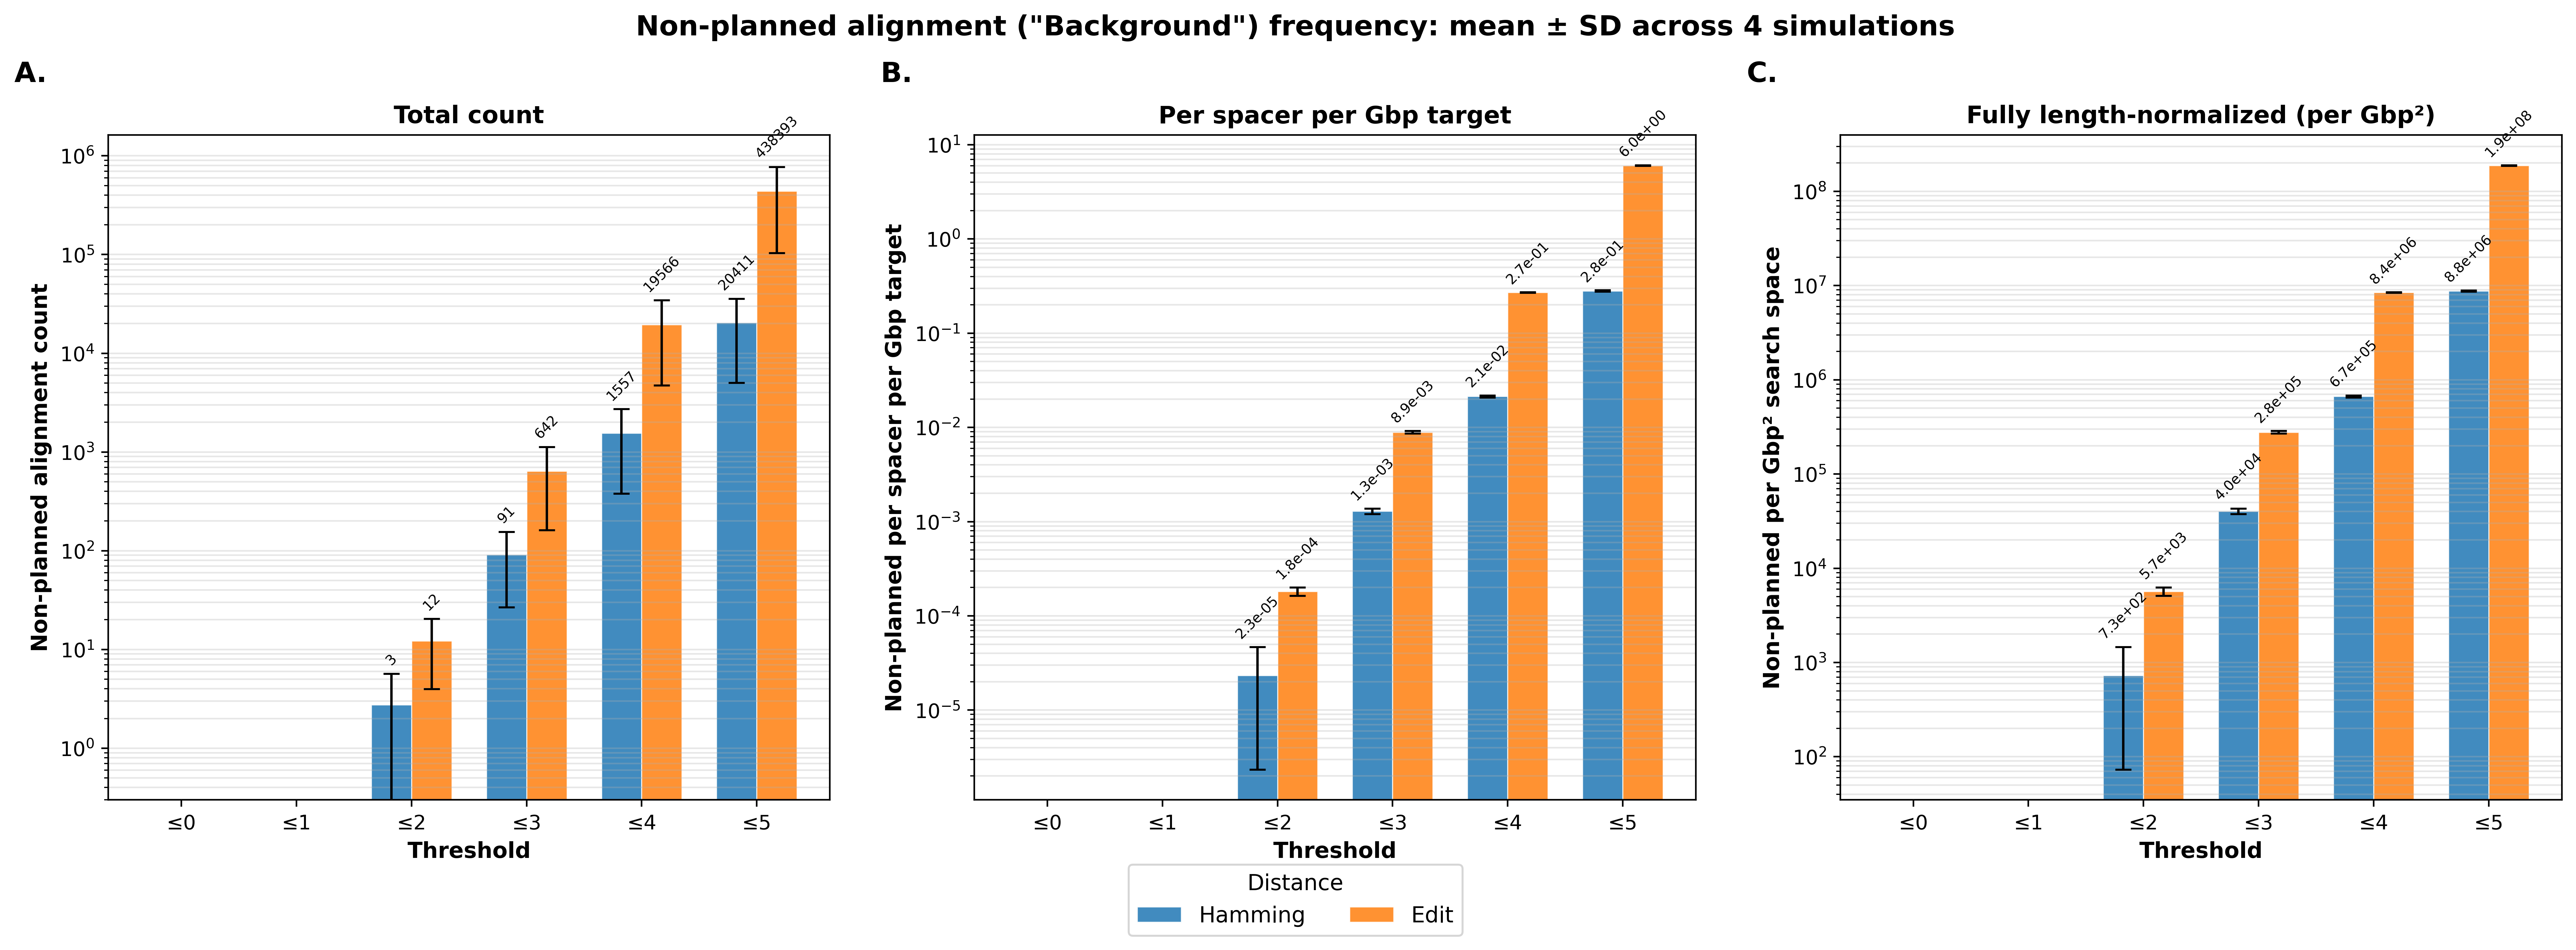
\includegraphics[keepaspectratio]{main_figures/Figure1_main_search_space_background_normalization.png}}

}

\caption{\label{fig-background-normalization}Non-planned alignment
(``background'') frequency: mean ± SD across 4 fully synthetic
simulations (50,000-100,000 spacers × 5,000-20,000 contigs). (A)
Absolute count of non-planned matches at each distance threshold (0-5).
(B) Non-planned matches normalized per spacer per Gbp of target
sequence. (C) Non-planned matches normalized per Gbp\^{}2 of total
search space (spacer-bp × contig-bp). Blue bars: hamming distance
(substitutions only). Orange bars: edit distance (substitutions +
indels). Error bars: standard deviation across simulations. At hamming
≤3, the per Gbp\^{}2 rate is approximately 40,000, while at edit ≤3 the
rate is approximately 270,000-290,000 (a 6-8 fold increase). Full
per-simulation breakdowns are provided in Supplementary Figure S9.}

\end{figure}%

Similarly, we use the semi-synthetic dataset (see
Section~\ref{sec-semi-synthetic}) to estimate non-planned match rates at
a scale analogous to the ``fraction\_1''. We note that this dataset size
was too prohibitive for the exhaustive and edit-distance based tools,
hence we rely on the aggregate of the non-exhaustive tools as a proxy
for the total number of non-planned matches, which is likely an
underestimate. Similarly, these results only estimate the hamming-based
non-planned match rates. Specifically, the total amount of non-planned
matches was 1 for 0 hamming threshold (i.e.~exact match), 49 for an
hamming distance of ≤1, 2,354 matches at ≤2 hamming distance, and 56,273
at ≤3 distance (see \hyperref[tbl-semisynthetic-hamming3]{Table 3} for
the results at hamming ≤3 compared to the fully synthetic simulation
mean.)

\begin{longtable}[]{@{}
  >{\raggedright\arraybackslash}p{(\linewidth - 6\tabcolsep) * \real{0.2500}}
  >{\raggedright\arraybackslash}p{(\linewidth - 6\tabcolsep) * \real{0.2500}}
  >{\raggedright\arraybackslash}p{(\linewidth - 6\tabcolsep) * \real{0.2500}}
  >{\raggedright\arraybackslash}p{(\linewidth - 6\tabcolsep) * \real{0.2500}}@{}}
\caption{Comparison of non-planned match rates at hamming distance ≤3
between fully synthetic simulations and the semi-synthetic dataset.
Absolute counts are not directly comparable due to different search
space sizes. Normalized metrics show the semi-synthetic dataset has
approximately 2.5× higher non-planned match rates, likely reflecting
biological sequence composition features in real spacers not fully
captured by simulated sequences (see Supplementary Table S7 and S8 for
the per-threshold
breakdowns).}\label{tbl-semisynthetic-hamming3}\tabularnewline
\toprule\noalign{}
\begin{minipage}[b]{\linewidth}\raggedright
\end{minipage} & \begin{minipage}[b]{\linewidth}\raggedright
Fully-Simulated (mean ± SD, n=4)
\end{minipage} & \begin{minipage}[b]{\linewidth}\raggedright
Semi-synthetic (real spacers)
\end{minipage} & \begin{minipage}[b]{\linewidth}\raggedright
Ratio
\end{minipage} \\
\midrule\noalign{}
\endfirsthead
\toprule\noalign{}
\begin{minipage}[b]{\linewidth}\raggedright
\end{minipage} & \begin{minipage}[b]{\linewidth}\raggedright
Fully-Simulated (mean ± SD, n=4)
\end{minipage} & \begin{minipage}[b]{\linewidth}\raggedright
Semi-synthetic (real spacers)
\end{minipage} & \begin{minipage}[b]{\linewidth}\raggedright
Ratio
\end{minipage} \\
\midrule\noalign{}
\endhead
\bottomrule\noalign{}
\endlastfoot
Non-planned matches (total) & 91.3 ± 64.5 & 56,273 & n/a (different
search space) \\
Per spacer per Gbp & 0.0013 ± 0.0001 & 0.00068 & 0.53× \\
Per Gbp2 search space & 40,314 ± 2,669 & 20,239 & 0.50× \\
\end{longtable}

The approximately 0.5-fold lower normalized rates in the semi-synthetic
dataset relative to fully synthetic simulations may stem from the real
spacer sequences having compositional features (conserved motifs,
non-uniform k-mer distributions, locus-specific GC variation) that alter
the rate of chance similarity. Therefore, these values should be
interpreted as qualitative indicators of relative (between edit vs
hamming and at increasing thresholds) background alignment rather than
exact predictive rates, as the simulated contigs only capture basic
sequence features (namely GC\% and length ranges), but not all
structural features of real viral genomes.

Given this estimation of chance similarity and background noise, we
selected hamming distance ≤3 as the primary threshold for most
subsequent analyses, but we acknowledge that for certain specific
research questions and scenarios, an edit distance may be more
appropriate, and we include some specific analyses to that effect.

\subsection{Tool performance across distance
thresholds}\label{sec-distance-performance}

\begin{figure}[H]

\centering{

\pandocbounded{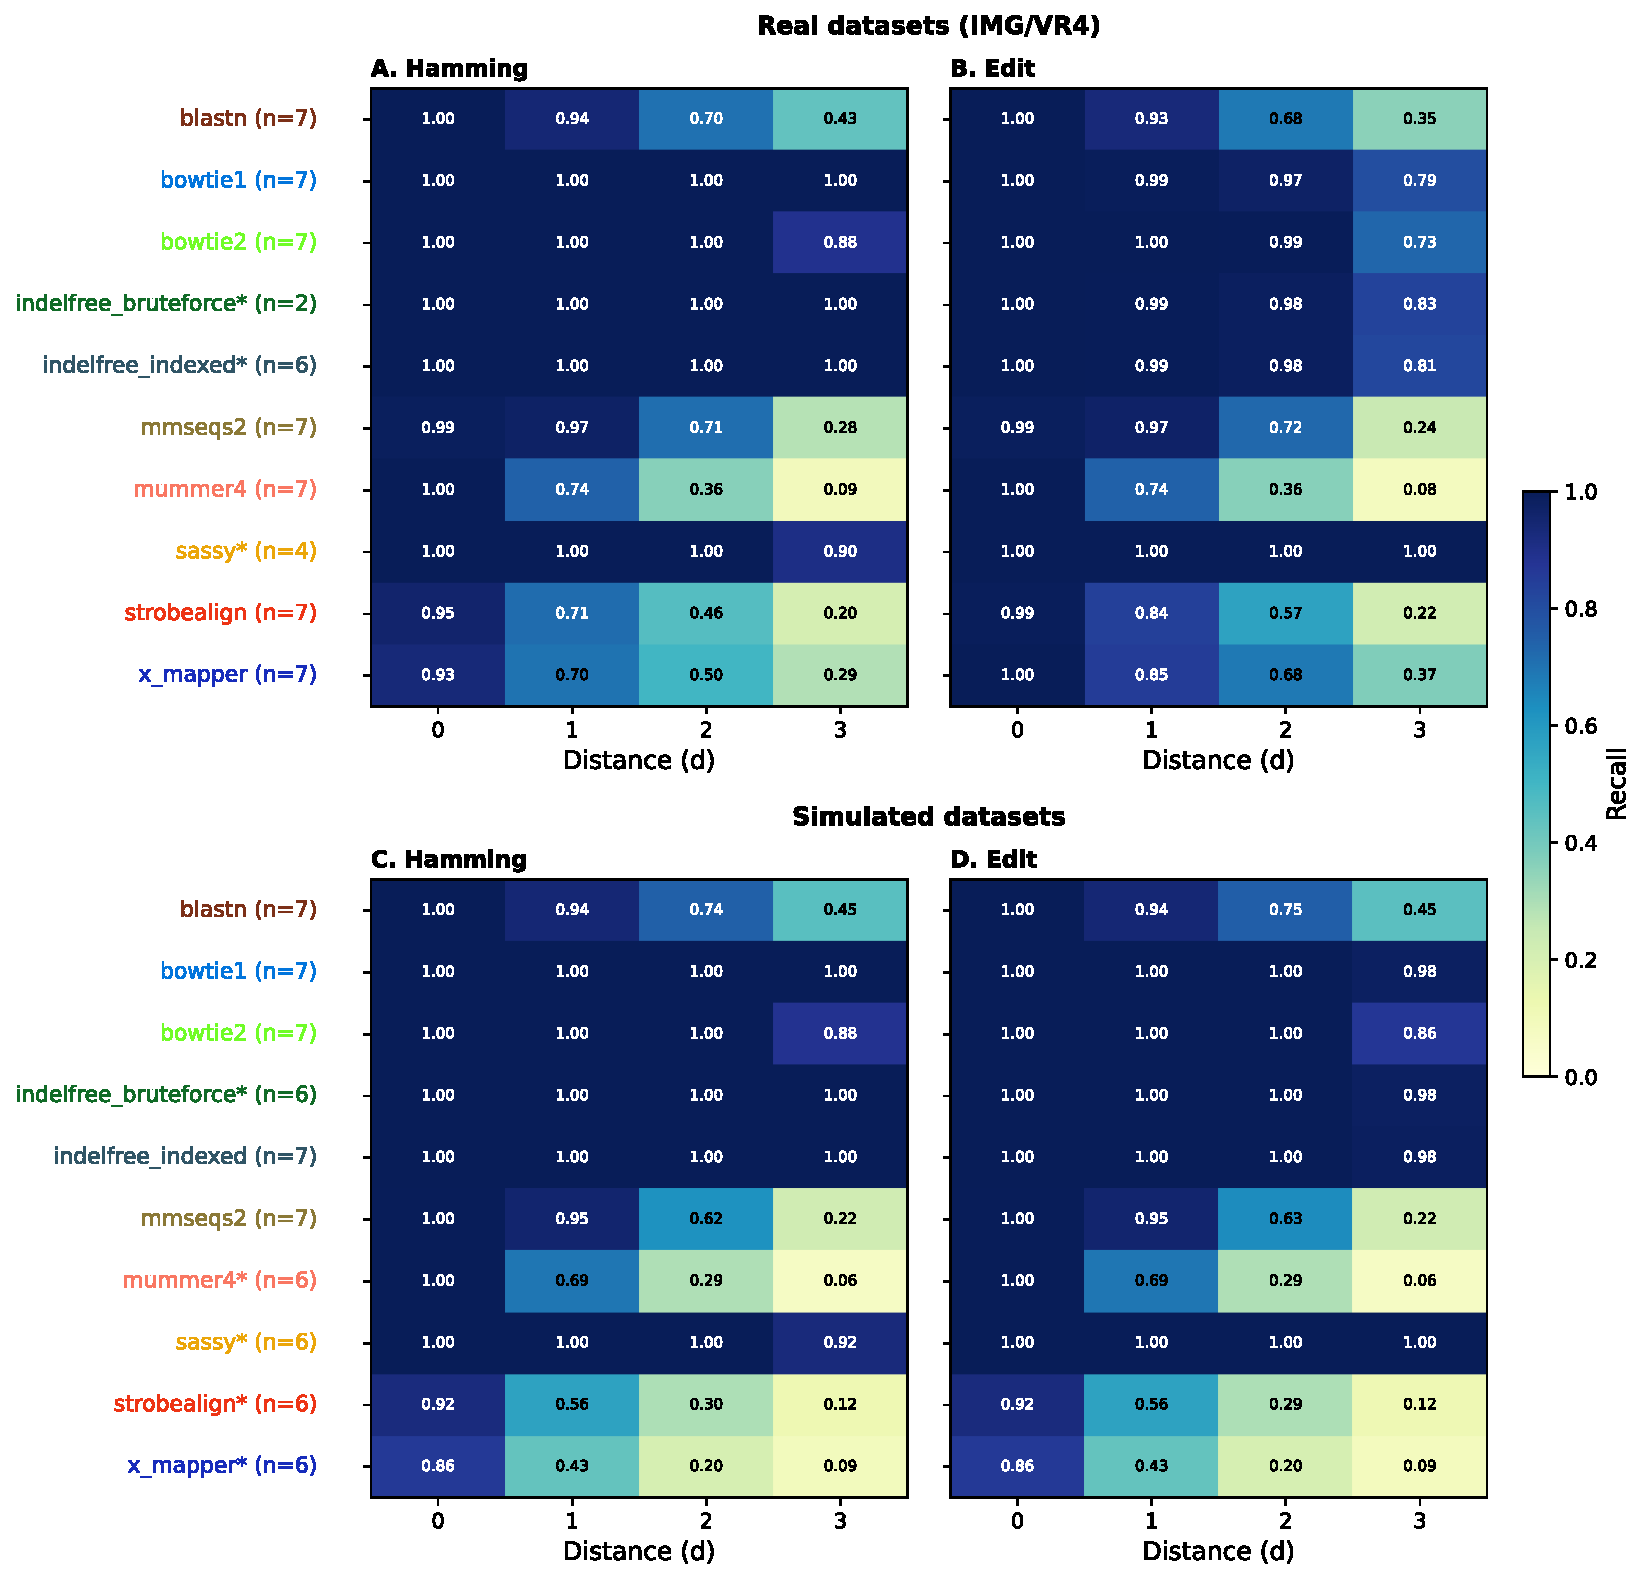
\includegraphics[keepaspectratio]{index_files/mediabag/main_figures/Figure2_main_heatmap_real_and_sim_hamming_edit_grid.pdf}}

}

\caption{\label{fig-tool-performance}Tool recall (detection fraction of
unique valid aligned regions) across distance thresholds. The upper row
shows IMG/VR4 (fractions) results and bottom row shows synthetic
datasets; columns compare hamming and edit distance analyses. An
asterisk ``*'' is noted after tools that did failed or timed out, and
the total number of successful runs (subsampled fraction for the IMG/VR
sets, and independent measurements for the simulated set) are noted in
brackets after each tool'name, and the value in each cell is the mean of
those run specific recall values. Note - the values are at exact
distance (unlike at a ``max'' distance), i.e.~regions that aligned with
distance n are not considered for distance n+1.}

\end{figure}%

We next evaluated the ability of individual tools to recover all valid
matches, summarized in \hyperref[fig-tool-performance]{Figure 2} as the
mean tool recall across a given spacer and target dataset type.

While we focus on hamming distance for the simulated datasets (i.e.~in
the current version, we only simulate substitutions, and not indels), we
included non-hamming based tools commonly used for sequence
searching/alignment. For both dataset types, we aggregate the tool
results and validate them under both hamming and edit distances
separately (see methods). We note however that this naturally penalizes
tools that might produce ``better'' alignments under their metric
(especially if the tool limits the reports to the best scoring alignment
per reference region), which might not align with the ``best''
(i.e.~minimal) hamming distance (for a given region). For example,
having a single gap in the middle of a spacer-target alignment could
produce a better (or valid/below certain distance value) alignment under
edit distance, but if the same aligned region is evaluated under hamming
distance, it is likely that half of the aligned region will include
multiple consecutive substitutions. Thus an important limitation here is
that more or less reported alignments per-tool under \textbf{all}
metrics, are not necessarily failures of the tool to detect the matches,
but rather a reflection of algorithmic differences in definitions. We
also note that in practice, the ability of some of the strictly-hamming
based tools (Bowtie1and indelfree in indexed mode) to report high recall
values under some of the measured edit-distance for the real-life
datasets, suggest that under these low (\textless=3) distances, there is
a large overlap between the actual alignable targets. The results
presented in figure 2 should therefore be informative once a specific
metric is selected.

With regards specific between-tool recall, performance varied
systematically with distance threshold. At distance 0 (exact matches),
multiple tools achieved recall above 0.95 on both simulated and real
datasets, including all tools except strobealign and x-mapper. As
mismatch tolerance increased, differences between tools became more
pronounced.

Across both simulated and real datasets, Bowtie1 (finished in allocated
time for all runs) and indelfree.sh (in index-mode, finished within
allocated time for all simulated run, and for 6 out of 7 of the
real-dataset fractions) remained the highest-recall heuristic tools at
hamming distance ≤3, while tools optimized for different mapping
contexts (notably StrobeAlign, MMseqs2 and MUMer4) showed larger recall
losses at higher mismatch levels. In edit-distance analyses, exhaustive
Sassy provided the expected upper bound when runs were computationally
feasible, while heuristic edit-capable tools showed variable sensitivity
depending on dataset scale and mismatch tolerance.

Performance patterns were consistent between simulated and real
datasets, though the smaller simulated dataset size and availability of
exhaustive tools on more synthetic data enabled more precise recall
measurement. A notable exception were strobealign, x-mapper and (to a
lesser degree, and in simulated runs only) mmseqs2, for which the
calculated recall rates varied between individual runs (see
Supplementary Figure S8). These variations were observed in both
simulated and real-dataset runs.

Complete per-tool, per-threshold recall values are provided in
Supplementary Table S6. In this regard, it is important to note that
within the allocated or available total CPU time per job, the largest
``real-dataset'' IMG/VR fraction amenable to the exhaustive tools was
1\% (sassy, edit) and 0.1\% (indelfree\_bruteforce, hamming; see section
below regarding computational resource usage for more details).

Pairwise tool comparisons measuring the set-difference of reported
alignments between two tools were consistent with these recall trends
(Supplementary Figure S1), indicating the same alignments were reported
by multiple tools at low distance values, and the number of
tool-specific differences quickly grew with increasing distances
considered.

\subsection{Computational Resource Requirements and
Scalability}\label{sec-resource-usage}

Computational resource requirements vary dramatically across tools,
reflecting fundamental differences in algorithmic approaches and
trade-offs between sensitivity and efficiency
(\hyperref[fig-resource-usage]{Figure~3}). Understanding these resource
requirements is essential for practical tool selection, particularly as
CRISPR spacer and viral databases continue growing rapidly.

\begin{figure}[H]

\centering{

\pandocbounded{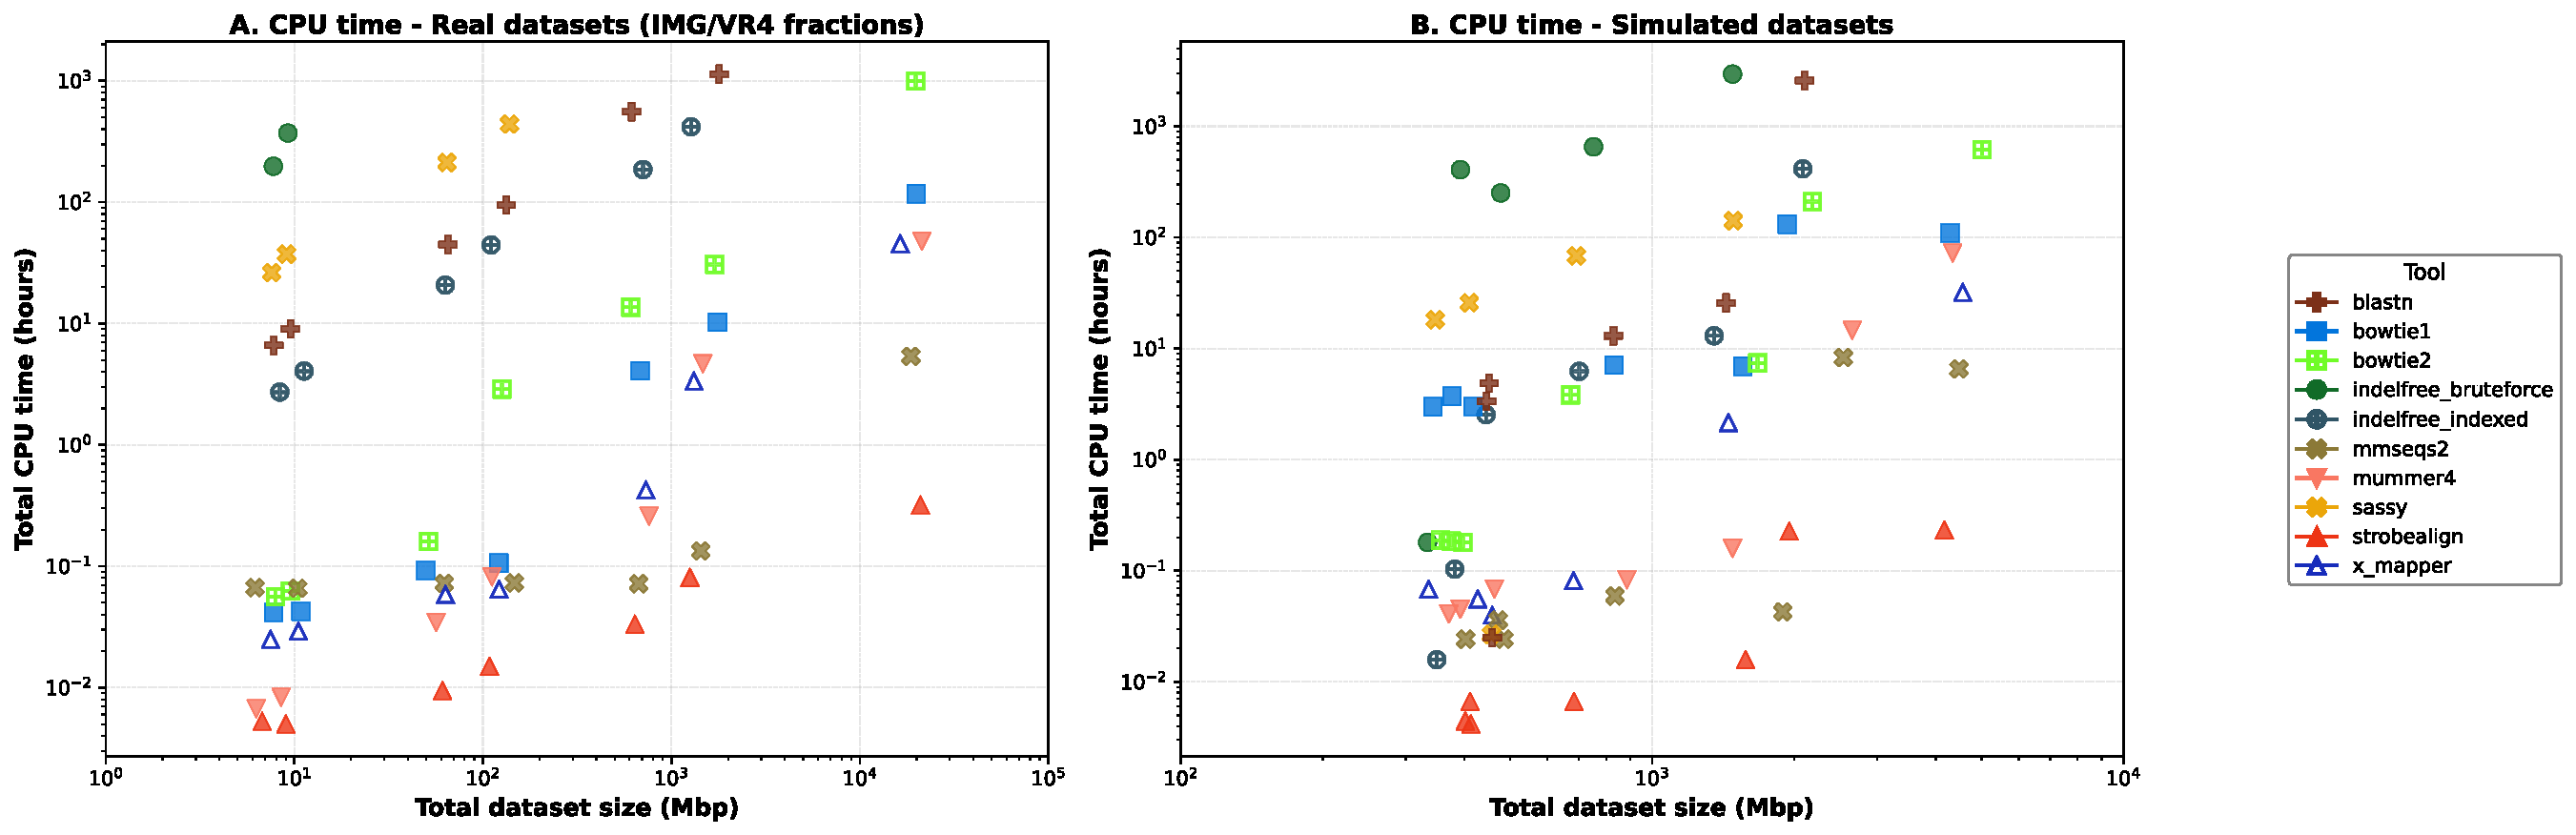
\includegraphics[keepaspectratio]{index_files/mediabag/main_figures/Figure3_main_resource_usage_cpu_2panel.pdf}}

}

\caption{\label{fig-resource-usage}Total CPU time scaling with dataset
size (log-log scale). (A.) Real IMG/VR4 subsampled datasets (fractions
0.001-1.0, approximately 10 Mbp to 18.9 Gbp target sequence). (B.)
Simulated datasets with varying numbers of spacers and contigs (see
Supplementary Table S4 for dataset details). Marker shape and color
encode tool identity. Note, x-axis ``jitter'' was applied to avoid
overlapping marker positions. BLASTn runtime for fraction\_1 was
extrapolated from partial completion (1.69M of 3.83M spacers processed
within the 72h wall time limit; see Supplementary Table S9 for all SLURM
accounting results).}

\end{figure}%

CPU-time trends in \hyperref[fig-resource-usage]{Figure 3} show large
differences in practical scalability, with exhaustive tools (Sassy
(orange ``x'' marker) and indelfree\_bruteforce (teal ``⏺'' marker))
typically requiring substantially longer runs even on smaller datasets.
Missing points indicate tool-dataset combinations that did not produce a
completed value for plotting (for example timeout, failed runs, or runs
excluded from the plotted subset); the corresponding SLURM-derived
records are provided in Supplementary Table S9, and the logs (stdout and
stderr) for all runs are available in the Zenodo repository.

Among heuristic methods, MMseqs2, StrobeAlign showed the most favorable
wall-time behavior across increasing dataset size, followed by MUMer4
and X-mapper. Bowtie1 and Bowtie2 typically had similar runtimes for the
same datasets, except for the smaller simulated runs where bowtie2
required considerably less time to complete. BLASTn and indelfree.sh in
indexed mode typically required substantially more time than the other
tools, and neither successfully finished processing the fraction\_1
(IMG/VR, real dataset) within the allocated 72-hour wall-time limit
(note -BLASTn was allowed to continue until completion solely for
comparison of results as it is the main tool historically used for
spacer-protospacer matching).\\
As expected, exhaustive tools were markedly slower; notably,
indelfree\_bruteforce remained computationally expensive even at
intermediate subsamples. Surprisingly, Sassy, despite being an
exhaustive edit-distance based tool, showed more favorable runtime than
indelfree\_bruteforce (a strictly hamming distance based tool),
reflecting that algorithmic constraints can be alleviated by dedicated
implementation optimizations.

With regards to memory usage (Supplementary Figure S7), SLURM peak
values differed by up to one to two orders of magnitude among tools.
This metric should be interpreted together with runtime because some
tools reduce memory pressure by partitioning reference data or
increasing disk I/O, which can increase wall time. Reported peak memory
for Java-based tools (x-mapper and BBMap-suite tools such as
indelfree.sh) may also be affected by JVM allocation behavior relative
to SLURM RSS accounting.

The paired real/simulated design also helps separate different scaling
effects. In simulated runs, both spacer and contig counts vary
(Supplementary Table S4), while in IMG/VR4 runs the spacer set is fixed
and only contig-side subsampling changes. This contrast suggests that,
for some tools, peak memory is influenced more strongly by index
structure and longest-contig properties than by total contig-set size
alone. Complete resource values and run-level details are provided in
Supplementary Table S9.

\subsection{Performance as a function of query (spacer) abundance in
reference}\label{sec-performance-as-a-function-of-query-spacer-abundance-in-reference}

In the fraction\_1 analysis, we observed occurrence-dependent
sensitivity effects in most tools, where spacers with very high
occurrence in the target set showed reduced recall (Supplementary Figure
S3). We corroborated this behavior with a dedicated high-insertion
simulation (ns\_500\_nc\_5000\_HIGH\_INSERTION\_RATE), where each spacer
was inserted between 100 to 2500 times in simulated contigs
(Supplementary Figure S2). The strongest degradations were tool-specific
and most were only visible at the highest occurrence bins. Importantly,
ultra-high occurrence spacers (\textgreater1000 occurrences) represented
a very small fraction of matched spacers (\textless0.01\%; Supplementary
Figure S6), so this effect is measurable but limited in overall
contribution to aggregate recall and likely to be limited in real-case
analyses.

\section{Discussion}\label{sec-discussion}

Our analysis across fully synthetic, semi-synthetic, and real IMG/VR4
datasets demonstrates that algorithmic design assumptions substantially
influence spacer-protospacer detection sensitivity. The quantitative
comparison of ten tools, including two exhaustive methods, enables
evidence-based recommendations while revealing systematic differences
rooted in the computational problems each tool was designed to solve.

\subsection{Distance metric choice and practical
thresholds}\label{sec-distance-thresholds}

The empirical non-planned match rates measured in this study provide
qualitative grounds for threshold selection. In the semi-synthetic
dataset (3,826,979 real spacers searched against 421,431 simulated
contigs), the number of validated non-planned matches rose sharply with
distance: 1 at exact match, 49 at hamming distance ≤1, 2,354 at ≤2, and
56,273 at ≤3 (\hyperref[tbl-semisynthetic-hamming3]{Table 3};
Supplementary Table S8). Analyses of fully synthetic datasets using
exhaustive tools further showed that edit distance ≤3 produced
approximately 6-8 fold more non-planned matches than hamming distance ≤3
at the same numeric threshold, and that the number of non-planned
matches quickly become overwhelming beyond distance cutoffs of ≤3
(thousands to tens of thousands in our simulations,
\hyperref[fig-background-normalization]{Figure 1}; Supplementary Table
S7). These quantitative observations, combined with the biological
evidence reviewed in the introduction for substitution-dominant phage
escape
mutations\autocite{Deveau2008,Semenova2011,Fineran2014,Schelling2023},
support hamming distance ≤3 as an appropriate default threshold for
spacer-protospacer matching in the context of host-MGE interaction
inference, in most scenarios.

The practical implications of these rates are scale-dependent. For small
datasets, such as a single or few phage genomes (total target sequence
well below approximately 1 Gbp) searched against spacers extracted from
several host genomes, the per-search-space-normalized rates suggest that
non-related matches at hamming ≤3 are infrequent. For large-scale host
assignment analyses where the total search space approaches or exceeds
the scale tested here, the expected number of non-planned matches should
inform downstream interpretation. At such scales, post-hoc filtering -
for example, requiring multiple supporting spacers per host-virus pair,
incorporating phylogenetic context, or applying stricter distance
thresholds - is warranted to mitigate the accumulation of chance
matches. Edit distance metrics may be appropriate under narrowly defined
conditions: when analyzing data from sequencing platforms with elevated
indel error rates (e.g., Oxford Nanopore R9 chemistry), when explicitly
characterizing escape mutation types in controlled experimental systems,
or when predicting gene-editing off-targets where multiple short indels
may still inform regions that could base-pair or lead to cleavage.
Outside of these scenarios, the substantially higher non-planned match
rates associated with larger edit distances (6-8 fold at ≤3) argue
against its routine use for inferring host-MGE interactions from natural
populations.

\subsection{Tool performance and algorithmic
considerations}\label{sec-tool-performance-discussion}

A central observation is that tools differ in recall rate not because of
implementation deficiencies, but because their algorithms solve
different computational problems. Edit/affine-based tools (Bowtie2,
Sassy) and hamming-based tools (Bowtie1, indelfree.sh,BLASTn-ungapped)
will, by definition, identify different match sets when applied at the
same numeric threshold, as they operate under different definitions.
This fundamental distinction must be considered when interpreting and
comparing results. Within the hamming distance analyses, Bowtie1
consistently achieved the highest recall among heuristic methods across
both dataset types and distance thresholds (Figure~2). Performance
patterns were notably consistent between simulated and real datasets
(Supplementary Figure S8), supporting the validity of our simulation
framework and suggesting these findings generalize across database
compositions.

At higher mismatch levels, differences between tools became more
pronounced. Tools originally designed for mapping short reads against
single-source reference assemblies (specifically StrobeAlign) showed
steeper recall declines, consistent with seed-selection heuristics that
penalize high-frequency k-mers or that assume reference uniqueness.
Similarly, we observed occurrence-dependent sensitivity effects (see
Section~\ref{sec-performance-as-a-function-of-query-spacer-abundance-in-reference}),
where spacers with many valid targets in the reference showed reduced
detection rates in most heuristic tools. While spacers with extremely
high occurrence frequency (\textgreater100 occurrences) represented a
negligible amount of the total matched spacers (\textless0.01\%)
(Supplementary Figure S6), the effect was measurable across a broader
range of occurrence frequencies and may matter for analyses specifically
targeting broadly conserved genomic regions.

The computational resource analysis reveals substantial differences in
scalability (\hyperref[fig-resource-usage]{Figure 3}; Supplementary
Figure S7). While index construction is often a one-time upfront cost,
we included it in the measured resource budget because it represents
real computational expenditure. Among heuristic tools, Bowtie1 combined
high recall with favorable runtime scaling, whereas BLASTn-short under
sensitivity-oriented parameters exceeded the 72-hour wall-time limit on
the full fraction\_1 dataset. The practical feasibility of exhaustive
tools depends strongly on dataset scale. For targeted analyses of
specific host-phage systems or comparisons among defined lineages, where
the total subject sequence is typically well below 1 Gbp and the number
of query spacers ranges from tens to thousands, exhaustive tools such as
Sassy and indelfree.sh bruteforce remain tractable and provide the
advantage of guaranteed complete detection. In contrast, for metagenomic
datasets where the combined contig set routinely exceeds 1 Gbp and
spacer sets may contain millions of sequences, the computational cost of
exhaustive search becomes prohibitive. For such analyses, heuristic
tools - particularly Bowtie1 - offer near-perfect recall at hamming
distance ≤3 with orders-of-magnitude lower resource requirements. Sassy,
notably, showed more favorable runtime than indelfree\_bruteforce
despite being an exhaustive edit-distance method, demonstrating that
dedicated algorithmic optimizations can substantially improve the
practical feasibility of exhaustive approaches. These resource
constraints directly affects feasibility of current and future viromics
studies, as spacer database size has been rapidly increasing - from
366,799 unique spacers in 2017\autocite{Shmakov_2017} to 1,173,006
unique spacers reported in 2021\autocite{Dion_2021} to 3,835,942 unique
spacers in 2023\autocite{camargo_img_vr4_2023}. Similarly, public virus
and MGE databases are growing rapidly, with large contributions from
metagenomic samples resulting in routine fold increases in the number of
predicted viral contigs\autocite{camargo_img_vr4_2023}.

\subsection{Biological interpretation of spacer-protospacer
matches}\label{sec-biological-interpretation}

Beyond tool performance, the biological interpretation of identified
matches requires careful consideration of several confounding scenarios.
Low-complexity regions, whether in the viral target set or in the spacer
set itself (where non-CRISPR repeated sequences may occasionally be
misclassified as spacers), can produce spurious matches independently of
tool choice. While certain tools employ internal filtering heuristics, a
separate complexity masking step using tools such as
DUST\autocite{Morgulis_2006} or similar approaches (e.g.~ldust, BBDuk)
prior to searching remains advisable. In our analysis, we applied light
filtration to the spacer database used in iPHoP, but observed that even
a ``cleaned'' spacer set (name of sourced file) may contain a handful of
very low complexity sequences.

Horizontal gene transfer (HGT) can spread conserved sequences across
unrelated MGEs, creating genuine sequence similarities that do not
reflect direct host-MGE interactions. Kosmopoulos et al.~described a
case where a transposon-mediated transfer of a phage lysin gene to the
host genome produced a verifiable sequence
match\autocite{Kosmopoulos_2023}, illustrating that an unknown fraction
of observed alignments may reflect HGT rather than CRISPR-mediated
interactions. Self-targeting events, where spacers match host genomic
sequences, have been estimated to have putative exogenous origin
(e.g.~prophages) in approximately 50\%\autocite{Stern_2010} to
80\%\autocite{Shmakov_2017} of cases, though the rate of true
non-defense self-targeting appears to be low\autocite{Shmakov_2017}.
Additional complexities include CRISPR systems encoded on
non-chromosomal replicons such as
plasmids\autocite{Maier_2018,Zhang_2025}, inter-species spacer
acquisition as described in some archaea\autocite{Turgeman_Grott_2018},
and phage-encoded mini-arrays that can interfere with host CRISPR
immunity\autocite{Shmakov_2023}.

The source and context of spacer data also merits consideration. Spacers
extracted from assembled CRISPR arrays carry additional information -
notably their position within the array and the observation that
co-located spacers originate from the same host. Mitrofanov et
al.\autocite{Mitrofanov2025} identified system subtype-dependent
patterns of spacer loss, and Vink et al.\autocite{Vink2021} reported
that most matched spacers in their analysis contained three or fewer
mismatched nucleotides, consistent with our general recommendation of
hamming distance ≤3. Vink et al.~also observed strand-targeting
preferences varying by CRISPR subtype (e.g.~Type I-E and Type II systems
preferentially target template strands), information that could enhance
post-search verification when combined with sequence orientation and
coding potential analysis.

\subsection{Study limitations}\label{sec-limitations}

Several aspects of this study merit explicit acknowledgment of
limitations. The synthetic datasets, while configured to match length
distributions and nucleobase frequencies of real data (Supplementary
Figure S4), do not fully capture all structural features of biological
sequences, including locus-specific composition biases, coding
constraints, and evolutionary signatures. The approximately 2.5-fold
higher normalized non-planned match rates observed in the semi-synthetic
dataset relative to the fully synthetic simulations (Table~2) likely
reflect such compositional features in real spacer sequences, and the
non-planned match rates reported here should accordingly be interpreted
as order-of-magnitude guides rather than precise predictive values.

Exhaustive tools (Sassy, indelfree.sh bruteforce) could not be run on
the full HQ benchmark dataset due to computational constraints. Our
comparisons on the largest datasets therefore rely on the aggregate of
heuristic tool results as a proxy for the complete positive set. For the
same reason, edit-distance-based exhaustive analysis was limited to the
smaller fully synthetic datasets. This tool-aggregate should therefore
be considered as an underestimate for the actual number of valid
alignments.\\
Another caveat lies in our current focus on hamming distance with
regards to simulated spacer occurrences. This means that
insertions/deletions are essentially ignored for most of our analysis.
While mutations related to CRISPR targeting are broadly expected to be
substitutions and indels have not been reported in this context, this
lack of reports does not equate lack of the phenomena occurring, and we
have enabled the option for the simulated spacers to vary in frequency
and type of mutations. We hope this would enable future versions of the
benchmark to estimate different tools' ability to identify these cases,
should they be established.

Additionally, tools were configured to maximize recall to the best of
our ability, based on tool documentation, github issue threads and
similar information sources. However, it is possible we either
misconfigured certain tools, or that exhaustively exploring all possible
parameter combinations would have yielded different results.\\
We also note that our analyses focused on assembled contigs from
Illumina-derived data; for other sequencing technologies or
raw-read-based workflows, additional considerations regarding sequencing
error profiles would apply.

\subsection{Conclusion}\label{sec-conclusion}

This work demonstrates that tool choice in spacer-protospacer matching
carries measurable consequences for downstream biological inference.
Based on the empirical evidence presented, we suggest Bowtie1 at hamming
distance ≤3 as a practical approach for large-scale analyses of host-MGE
interactions through CRISPR spacers, given its combination of high
sensitivity, computational efficiency, and consistency across dataset
scales. For analyses requiring tolerance beyond 3 substitutions,
indelfree.sh in indexed mode extends the hamming distance range without
incurring a considerable elevated non-planned match rates, such as those
observed for edit distance above 3. Of note, exhaustive tools (such as
Sassy for edit and indelfree bruteforce) remain appropriate for small
scale analyses - including experimental studies of individual host-phage
systems (e.g.~one or several phages and spacers from several arrays), or
even medium-scale analysis (e.g.~lineage-specific comparison such as all
arrays from a specific bacterial genus and all their known phages).
Additionally, the exhaustive tools can simplify result validation of
heuristic tool outputs - where the total subject sequence is modest or
if computational resources permit complete enumeration. For large scale
analysis, such as using complete public spacer and large virus
databases, a combination of heuristic tools currently appears as the
only possible option.\\
Edit distance metrics may be warranted under specific conditions: when
analyzing low-accuracy long-read data where sequencing-induced indels
cannot be excluded, when investigating escape mutation mechanisms in
controlled experimental systems where the mutation type itself is
informative (and could be verified experimentally post-hoc), or when
working in gene-editing off-target prediction contexts where gapped
alignments have established biological relevance (such as RNA structure
importance for activity). For all other cases, hamming distance ≤3
appears to capture the dominant mode of protospacer divergence
(substitutions) as currently reported in literature, while maintaining a
favorable ratio of genuine to non-planned matches. We emphasize that
regardless of tool choice, post-hoc verification of alignment quality,
complexity filtering, and contextual biological analysis remain
important components of any spacer-protospacer matching workflow in the
context of host range prediction.

\section{Code and data availability}\label{sec-code-data}

All code generated for this study can be found in the git repository:
\href{https://github.com/UriNeri/spacer_matching_bench}{\emph{github.com/UriNeri/spacer\_matching\_bench}}.
All data generated in this project (tool results and the analysed
datasets, any sequence data, SLURM logs etc) are available on
Zenodo\autocite{zenodo_doi}.

\section{Acknowledgements}\label{sec-acknowledgements}

Work conducted by the U.S. DOE Joint Genome Institute
(https://ror.org/04xm1d337) (SR, UN, APC and BB), a DOE Office of
Science User Facility, is supported by the Office of Science of the U.S.
DOE operated under Contract DE-AC02-05CH11231. indelfree.sh, bbmap.sh
and other bbtools suite tools are available and documented via
\href{http://bbmap.org}{\emph{bbmap.org}}.

We would like to thank the following people for their helpful feedback
and suggestions: Uri Gophna, Georg Rath, and Ragnar Groot Koerkamp for
valuable discussions on distance metrics and tool performance.


\printbibliography



\end{document}
